% Latex template: mahmoud.s.fahmy@students.kasralainy.edu.eg
% For more details: https://www.sharelatex.com/learn/Beamer

\documentclass{beamer}					% Document class
\geometry{papersize={15cm,10cm}}

\setbeamertemplate{footline}[text line]{%
  \parbox{\linewidth}{\vspace*{-8pt}\hfill\hfill\insertpagenumber}}
\setbeamertemplate{navigation symbols}{}

\usepackage[english]{babel}				% Set language
\usepackage[utf8x]{inputenc}			% Set encoding

\mode<presentation>						% Set options
{
  \usetheme{default}					% Set theme
  \usecolortheme{default} 				% Set colors
  \usefonttheme{default}  				% Set font theme
  \setbeamertemplate{caption}[numbered]	% Set caption to be numbered
}

% Uncomment this to have the outline at the beginning of each section highlighted.
%\AtBeginSection[]
%{
%  \begin{frame}{Outline}
%    \tableofcontents[currentsection]
%  \end{frame}
\usepackage{graphicx}					% For including figures
\usepackage{booktabs}					% For table rules
\usepackage{hyperref}	
\usepackage{tikz-network}				% For cross-referencing
\usepackage[absolute,overlay]{textpos}
\usepackage{bm}
\usepackage[font=small,labelfont=bf]{caption}				% For cross-referencing
\usepackage{comment}

\title{Advancing super resolution microscopy for quantitative in-vivo imaging of chromatin nanodomains}	% Presentation title
\author{Clayton W. Seitz}								% Presentation author
\date{\today}									% Today's date	

\setbeamertemplate{footline}{
    \hbox{%
    \begin{beamercolorbox}[wd=\paperwidth,ht=3ex,dp=1.5ex,leftskip=2ex,rightskip=2ex]{page footer}%
        \usebeamerfont{title in head/foot}%
        \insertshorttitle \hfill
            \insertsection \hfill
        \insertframenumber{} / \inserttotalframenumber
    \end{beamercolorbox}}%
}

\AtBeginSection[]{
  \begin{frame}
  \vfill
  \centering
  \begin{beamercolorbox}[sep=8pt,center,shadow=true,rounded=true]{title}
    \usebeamerfont{title}\insertsectionhead\par%
  \end{beamercolorbox}
  \vfill
  \end{frame}
}

\begin{document}

% Title page
% This page includes the informations defined earlier including title, author/s, affiliation/s and the date
\begin{frame}
  \titlepage
\end{frame}

\begin{frame}{Outline}
    \tableofcontents
\end{frame}



% The following is the most frequently used slide types in beamer
% The slide structure is as follows:
%
%\begin{frame}{<slide-title>}
%	<content>
%\end{frame}




\section{Introduction}

\begin{frame}{Chromatin organization and super resolution imaging}
\begin{textblock*}{12cm}(1.5cm,1.5cm)
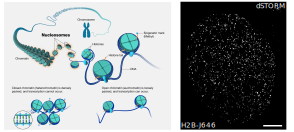
\includegraphics[width=12cm]{Intro2}
\end{textblock*}
\begin{textblock*}{12cm}(1.0cm,7.5cm)
\begin{itemize}
\item Chromatin has a hierarchical structure, fundamental unit is the nucleosome
\item We study chromatin organization with SMLM
\end{itemize}
\end{textblock*}

\end{frame}

\begin{frame}{Direct stochastic optical reconstruction microscopy (dSTORM)}
\begin{textblock*}{13cm}(1.0cm,1.5cm)
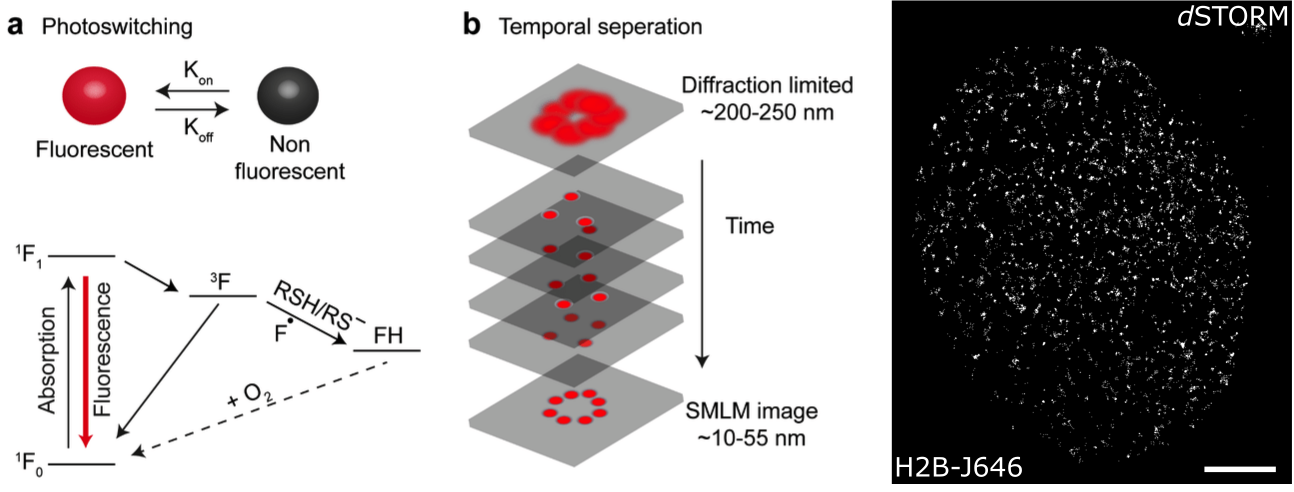
\includegraphics[width=\textwidth]{Intro.png}
\end{textblock*}
\begin{textblock*}{\textwidth}(1.0cm,7.5cm)
\begin{itemize}
\item SMLM techniques are diffraction-unlimited
\item Photoswitching enables resolution of emitters below the diffraction limit
\end{itemize}
\end{textblock*}
\end{frame}

\begin{frame}{Single molecule localization microscopy and its applications}
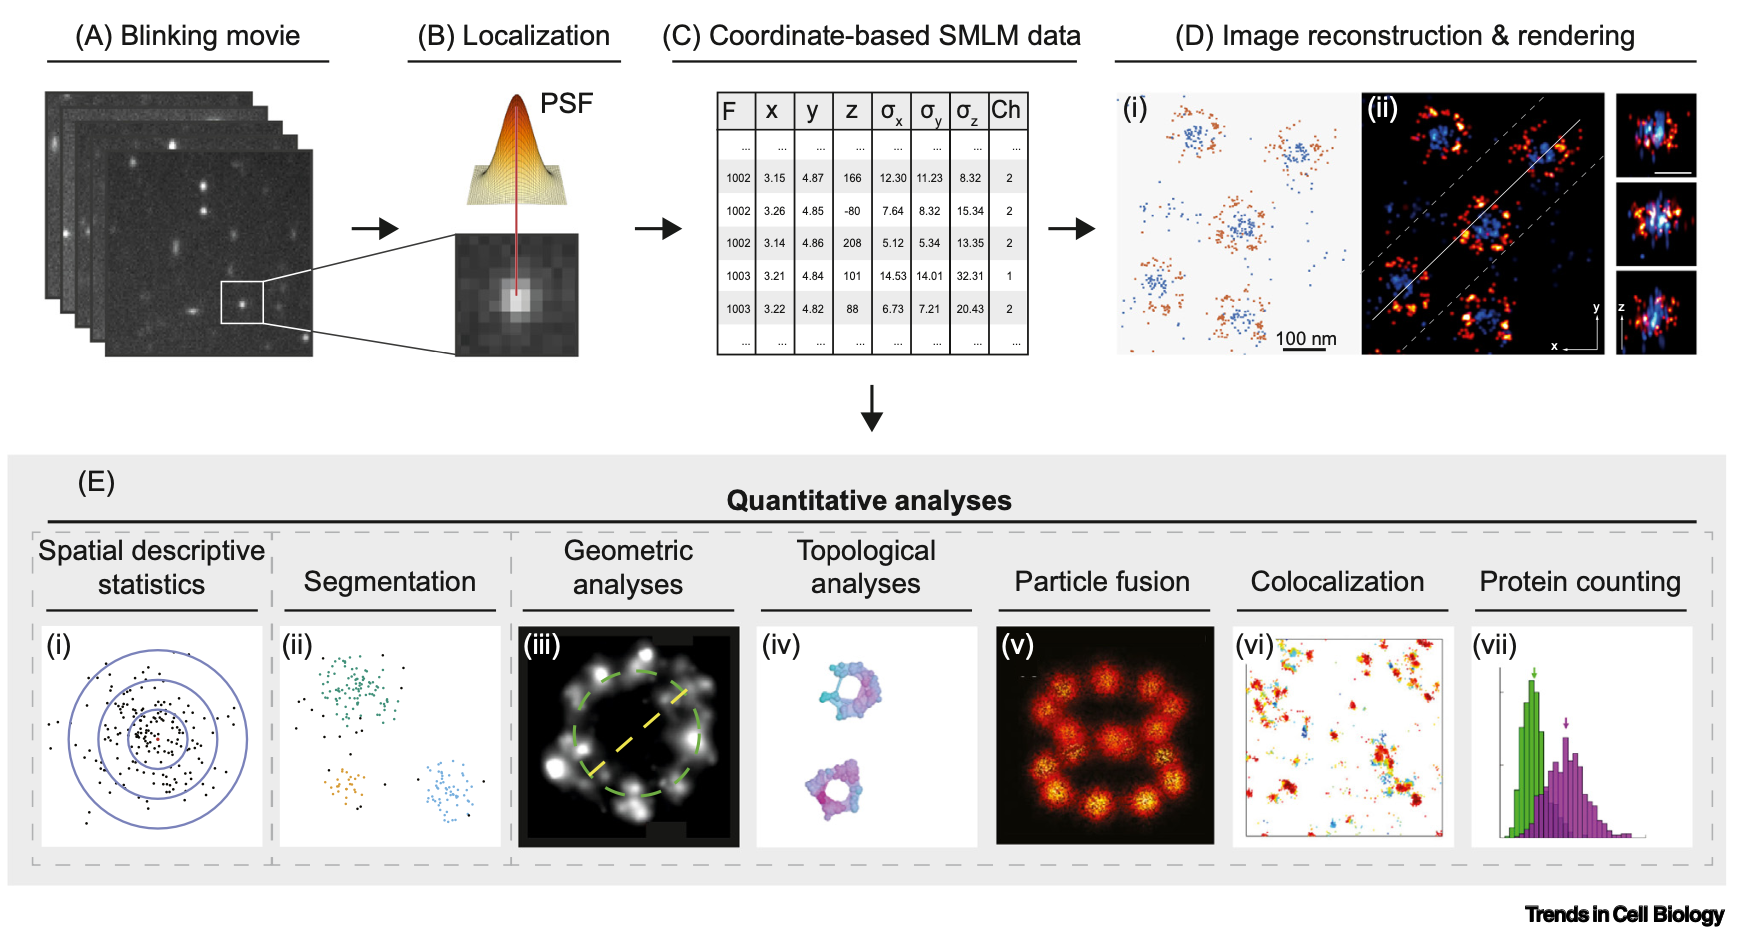
\includegraphics[width=\textwidth]{Apps}
\textit{Wu et al. Quantitative Data Analysis in Single-Molecule Localization Microscopy.}
\end{frame}

\section{Theory of SMLM} 

\begin{frame}{Single molecule localization microscopy}

Modeling the point spread function permits sub-pixel localization 

\begin{textblock*}{8cm}(6.5cm,2.0cm)
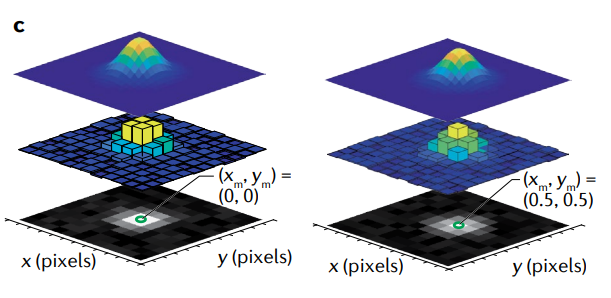
\includegraphics[width=\textwidth]{Model.png}
\end{textblock*}

\begin{textblock*}{2cm}(1cm,2.0cm)
\begin{align*}
\mu_{k} &= i_{0}\int_{\mathrm{k}}h_{\theta}(x_{0},y_{0})dxdy\\
i_{0} &= g_{k}\textcolor{red}{\eta} \textcolor{cyan}{N_{0}}\textcolor{blue}{\Delta} 
\\
\textcolor{red}{\eta} &- \mathrm{quantum\; efficiency}\\
\textcolor{cyan}{N_{0}} &- \mathrm{photon\; emission\; rate}\\
\textcolor{blue}{\Delta} &- \mathrm{exposure\; time}
\end{align*}
\end{textblock*}

\vspace{2in}

Assume $N_{0}$ is constant over $\textcolor{blue}{\Delta}$ (homogeneous Poisson)

\begin{equation*}
\theta^{*} = \underset{\theta}{\mathrm{argmax}}\prod_{k}P(H_{k}|\theta)= \underset{\theta}{\mathrm{argmin}}-\sum_{k}\log P(H_{k}|\theta)
\end{equation*}

\end{frame}

\begin{frame}{CMOS readout noise limits SMLM}

\begin{figure}
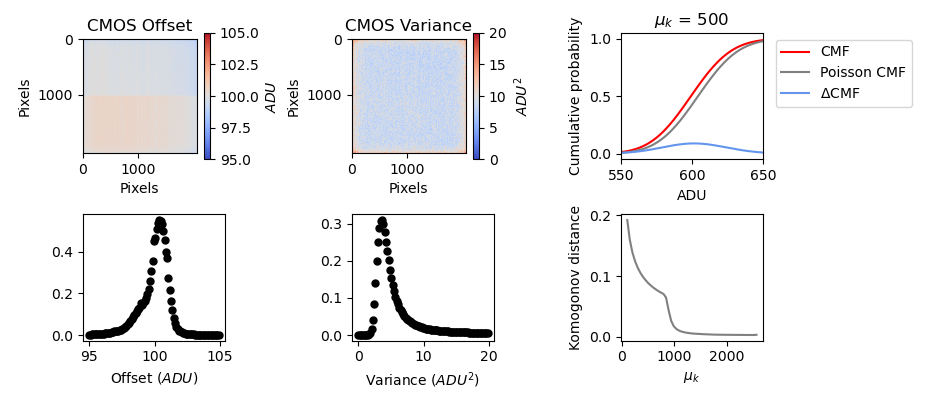
\includegraphics[width=13cm]{Noise.png}
\end{figure}

\begin{align}
P(H_{k}|\theta) &=  A\sum_{q=0}^{\infty} \frac{1}{q!}e^{-\mu_{k}}\mu_{k}^{q}\frac{1}{\sqrt{2\pi}\sigma_{k}}e^{-\frac{(H_{k}-g_{k}q-o_{k})}{2\sigma_{k}^{2}}}
\end{align}


$P(H_{k}|\theta)$ can be approximated as Poisson at high signal-to-noise ($\mathrm{SNR}$)
 
\end{frame}

\begin{frame}{Localization uncertainty in SMLM}
\begin{textblock*}{4cm}(1.0cm,1.0cm)
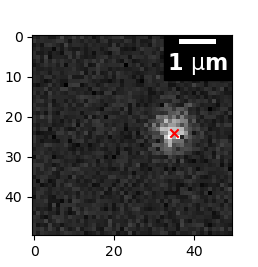
\includegraphics[width=4cm]{MCMC/Figure_1.png}
\end{textblock*}
\begin{textblock*}{4cm}(1.0cm,5cm)
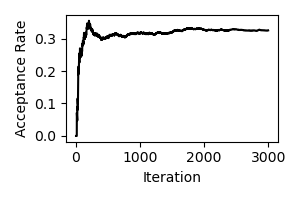
\includegraphics[width=4cm]{MCMC/Figure_2.png}
\end{textblock*}
\begin{textblock*}{9cm}(5cm,1.0cm)
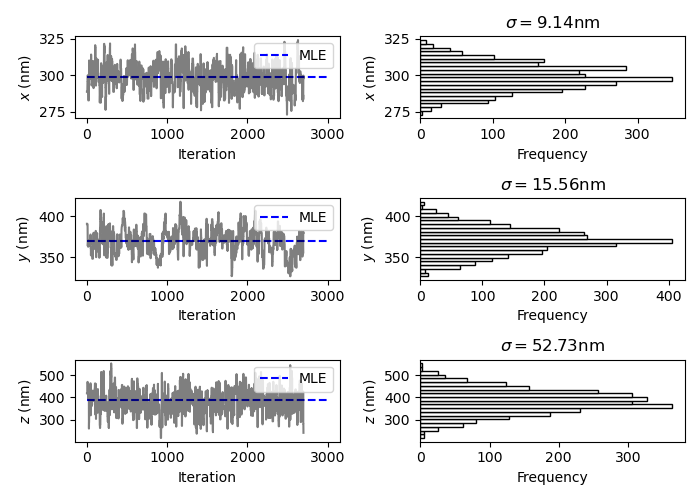
\includegraphics[width=9cm]{MCMC/Figure_3.png}
\end{textblock*}
\begin{textblock*}{13cm}(0.5cm,8cm)
\begin{itemize}
\item Sampling the coordinates $\theta$ gives uncertainty estimates
\end{itemize}
\end{textblock*}

\end{frame}


\begin{comment}
\begin{frame}
\frametitle{Super resolution with photoswitching of rhodamines}

\begin{figure}
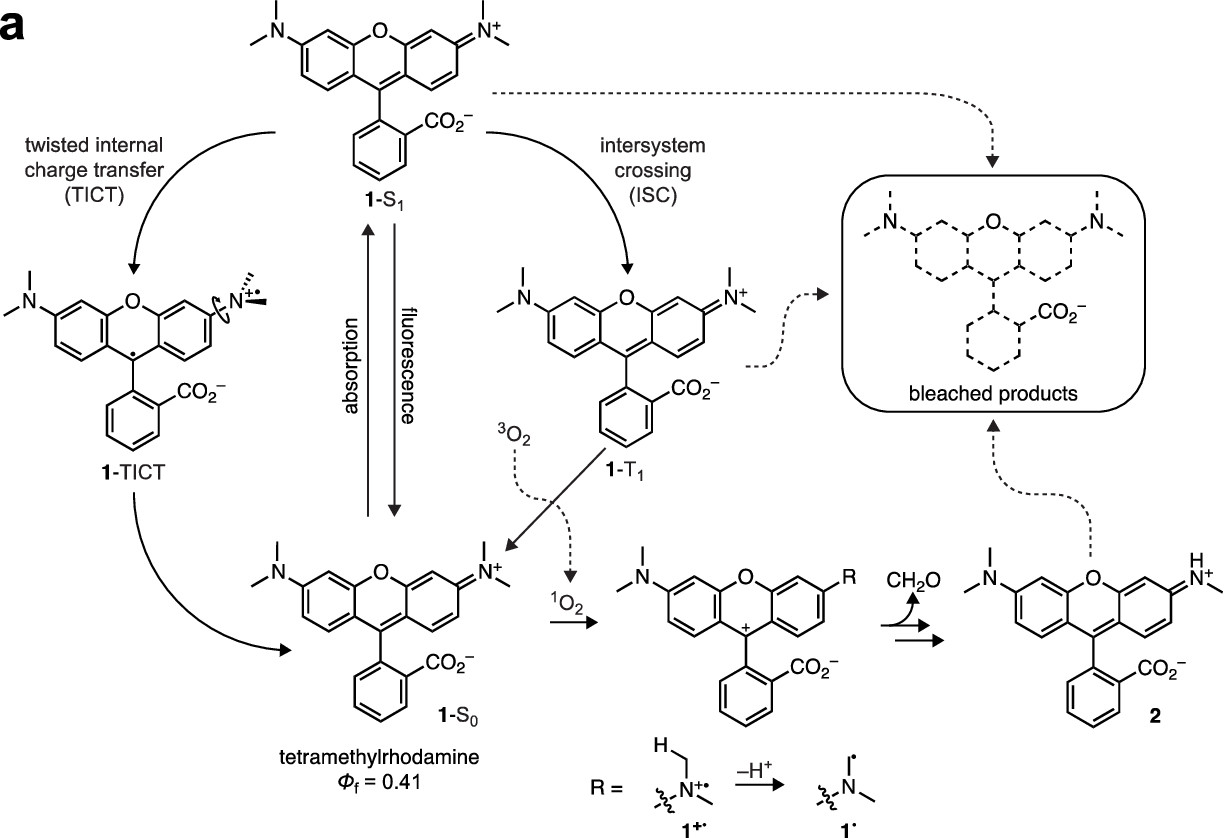
\includegraphics[width=10cm]{Rhodamines.png}
\end{figure}
\begin{itemize}
\item  Reduction of the T1 state yields a dark, long-lived, and stable radical state
\end{itemize}
\end{frame}
\end{comment}

\begin{comment}
\begin{frame}
\frametitle{Direct stochastic optical reconstruction microscopy}

\begin{figure}
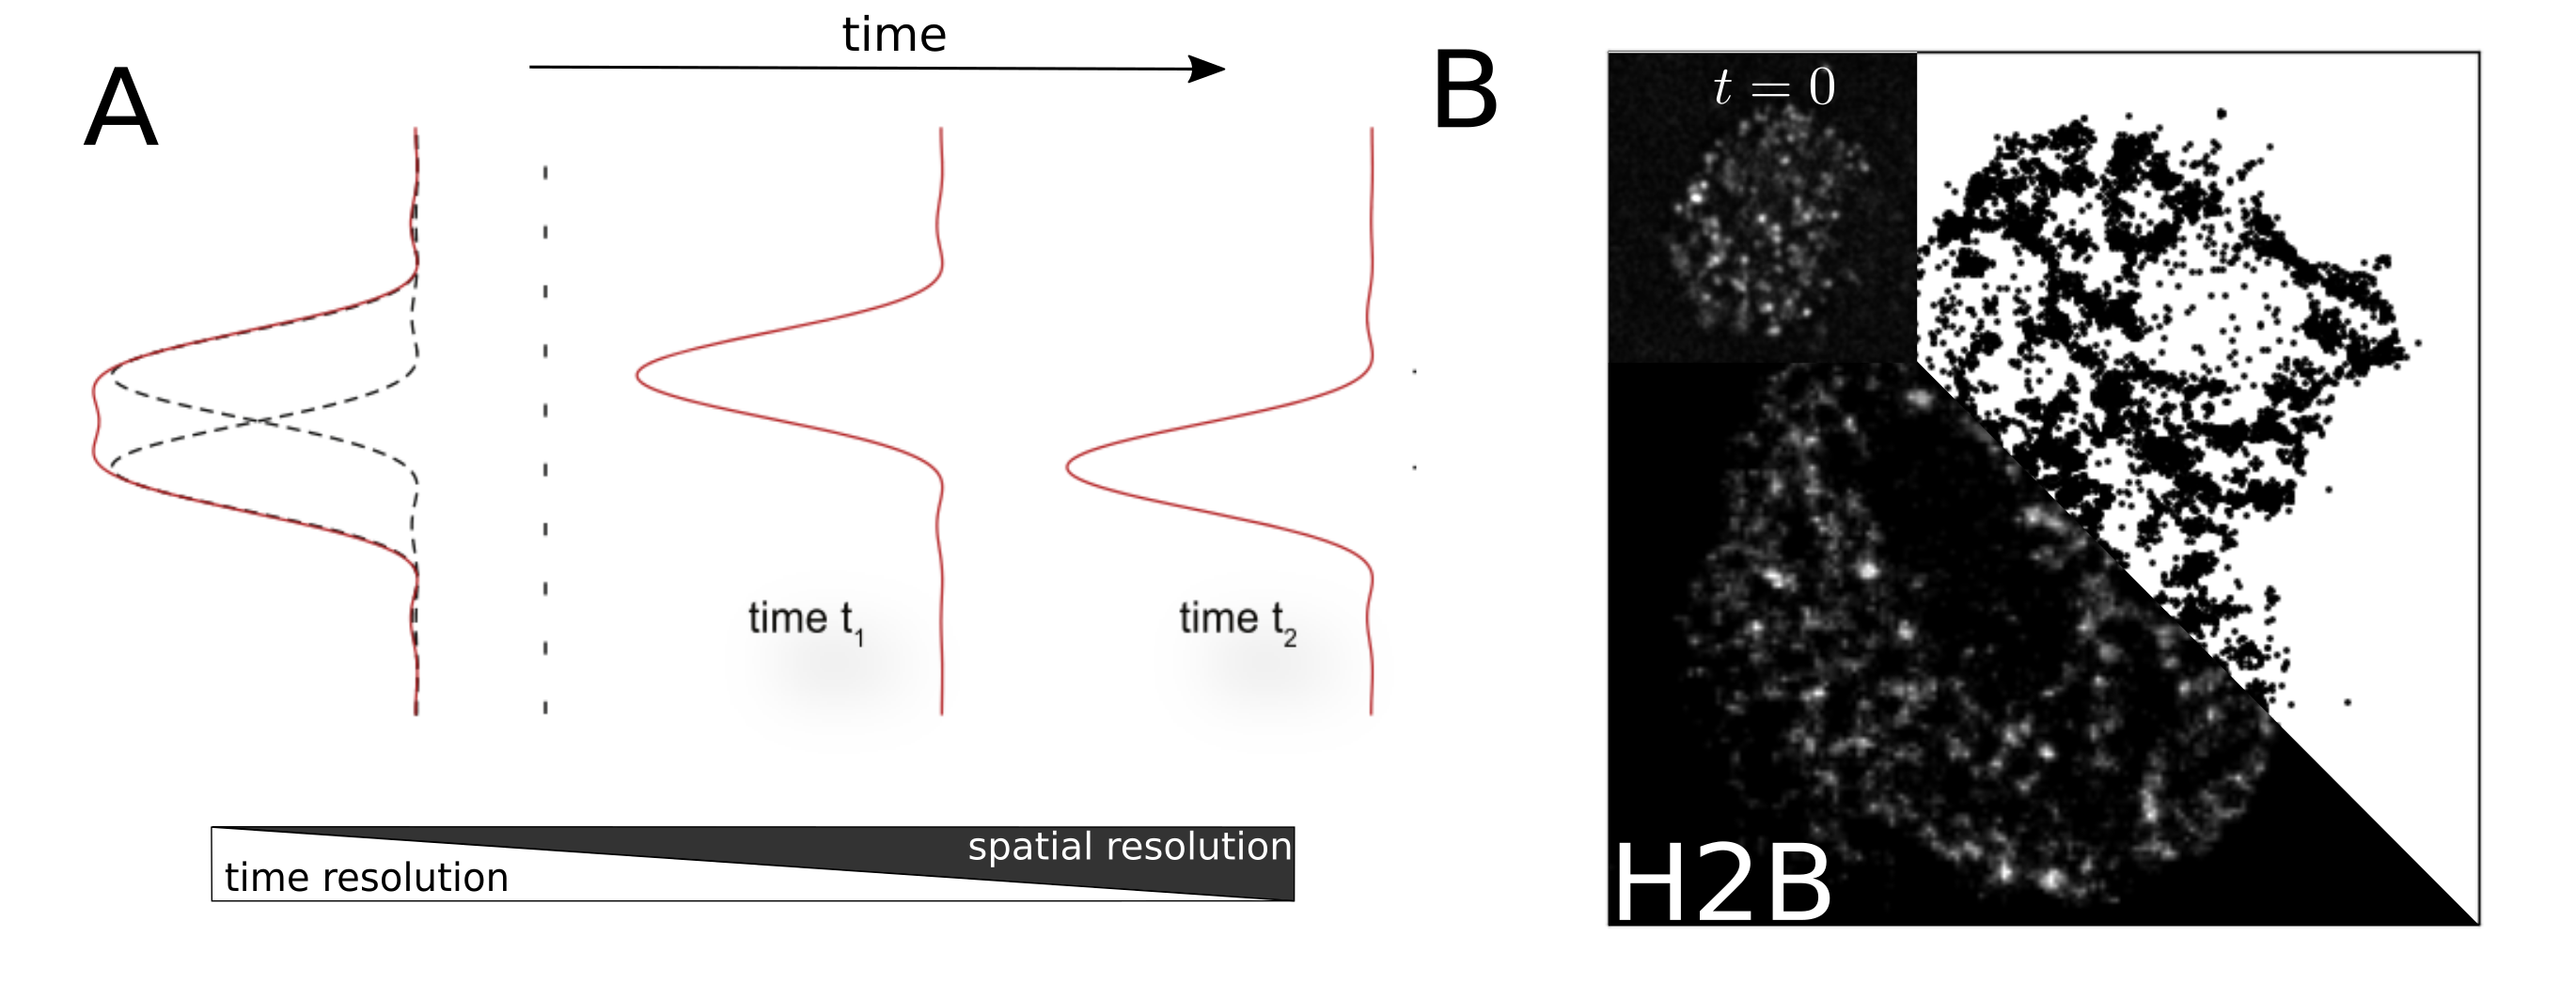
\includegraphics[width=13cm]{Concept.png}
\end{figure}

\begin{itemize}
\item Photoswitching enables resolution of emitters in time rather than space
\item Presents a tradeoff between spatial and temporal resolution
\end{itemize}

\end{frame}
\end{comment}


\begin{frame}{The definition of resolution in SMLM}
\begin{textblock*}{13cm}(1cm,1.25cm)
\begin{itemize}
\item We can view dSTORM as sampling from a density
\end{itemize}
\end{textblock*}
\begin{textblock*}{9cm}(3cm,2.0cm)
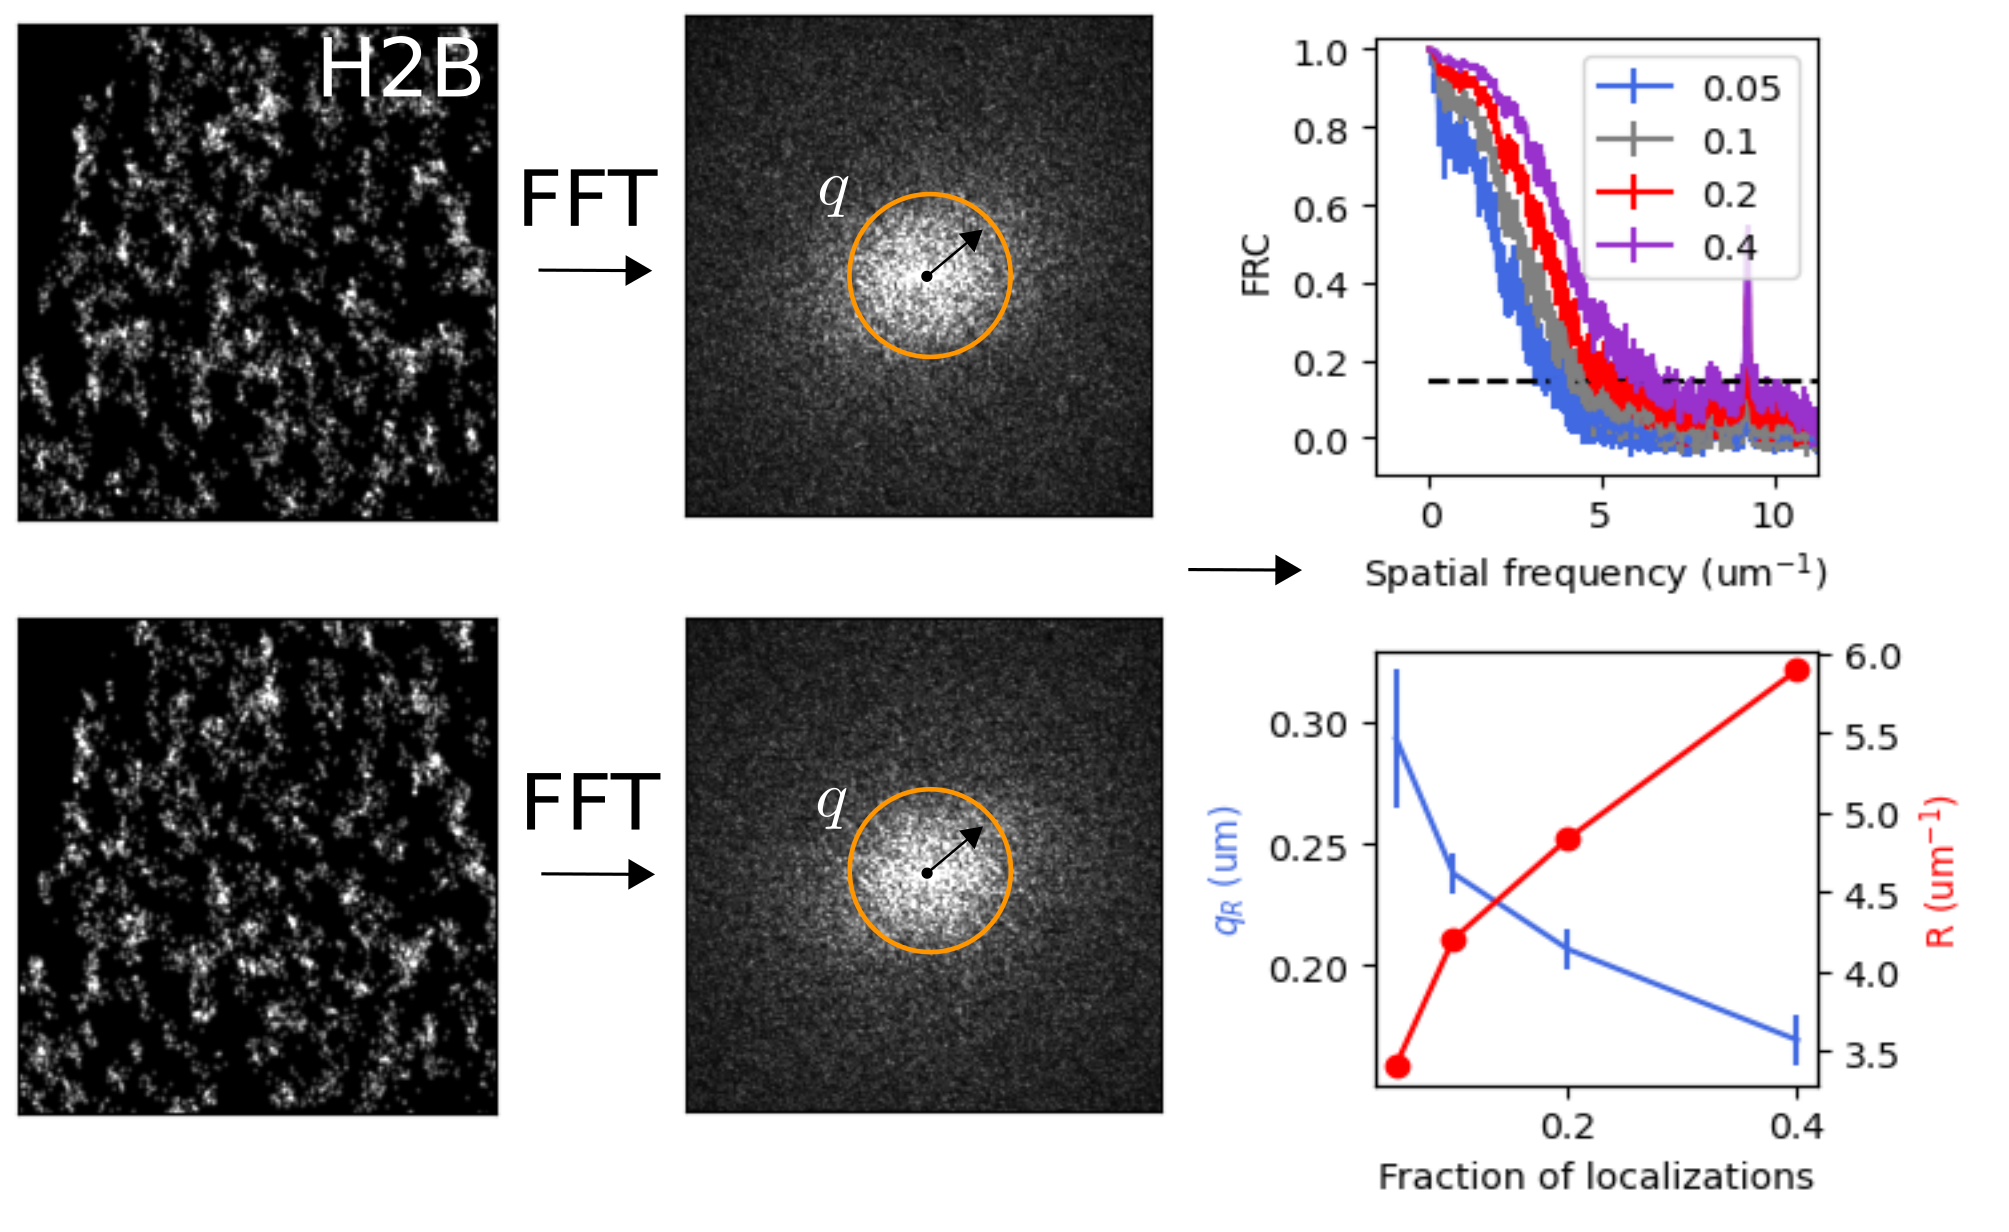
\includegraphics[width=9cm]{FRC.png}
\end{textblock*}
\begin{textblock*}{8cm}(3cm,7.5cm)
\begin{equation*}
\mathrm{FRC}(q) = \frac{\sum_{\vec{q}\in\mathrm{circle}}\tilde{f_{1}}(\vec{q})\tilde{f_{2}}(\vec{q})^{*}}{\sqrt{\sum_{\vec{q}\in\mathrm{circle}}|f_{1}(\vec{q})|^{2}}\sqrt{\sum_{\vec{q}\in\mathrm{circle}}|f_{2}}(\vec{q})|^{2}}
\end{equation*}
\end{textblock*}
\end{frame}

\begin{frame}{The definition of resolution in SMLM}
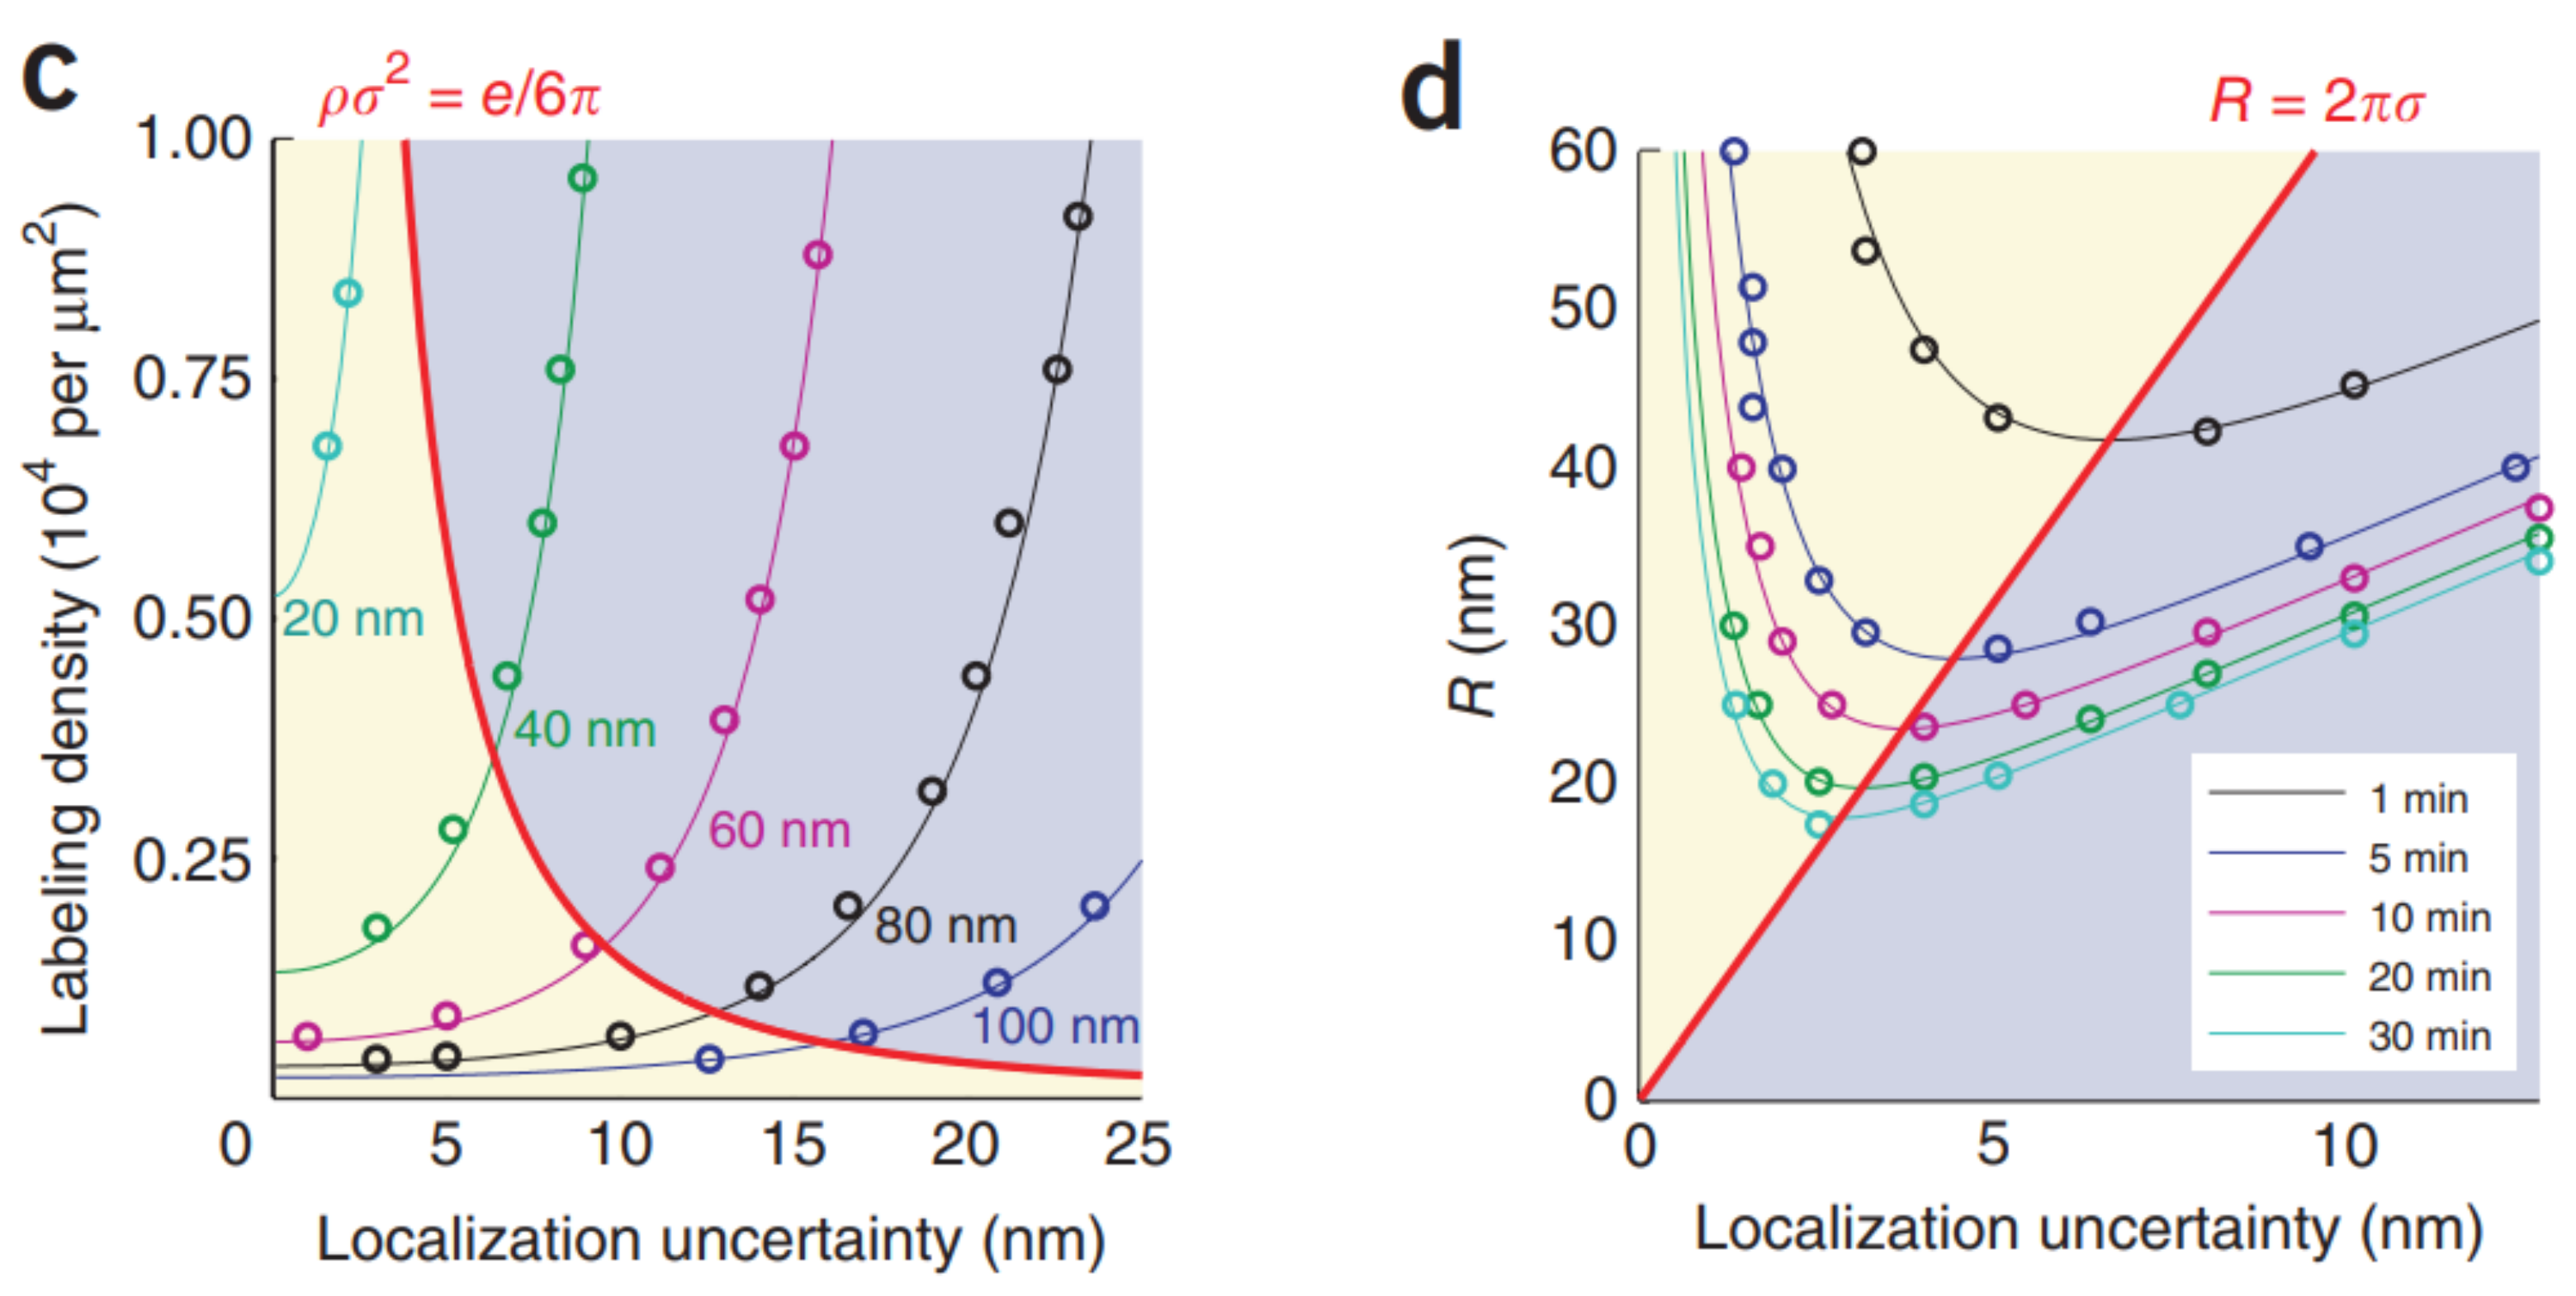
\includegraphics[width=\textwidth]{Spatial.png}
\vspace{0.025in}
\textit{Nieuwenhuizen et al. Measuring image resolution in optical nanoscopy.}
\vspace{0.05in}
\begin{itemize}
\item Increased localization uncertainty requires higher density for same resolution
\item Longer acquisitions have higher resolution
\end{itemize}

\end{frame}

\section{Enhanced SMLM with photon statistics}

\begin{frame}{Single photon avalanche diode (SPAD) cameras}

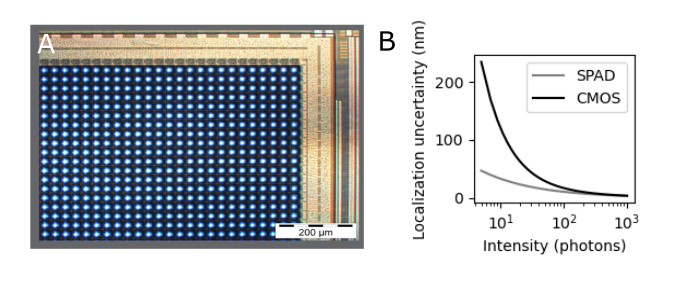
\includegraphics[width=12cm]{SPAD-Intro.png}\\
\textit{(A) Courtesy of Pi imaging technologies}
\vspace{0.05in}
\begin{itemize}
\item Imaging in low light conditions (near zero readout noise)
\item Reduced quantum efficiency ($\eta\approx 0.5$), but frame rates up to 1MHz
\end{itemize}


\end{frame}

\begin{frame}{High speed imaging for enhanced SMLM}
\begin{figure}
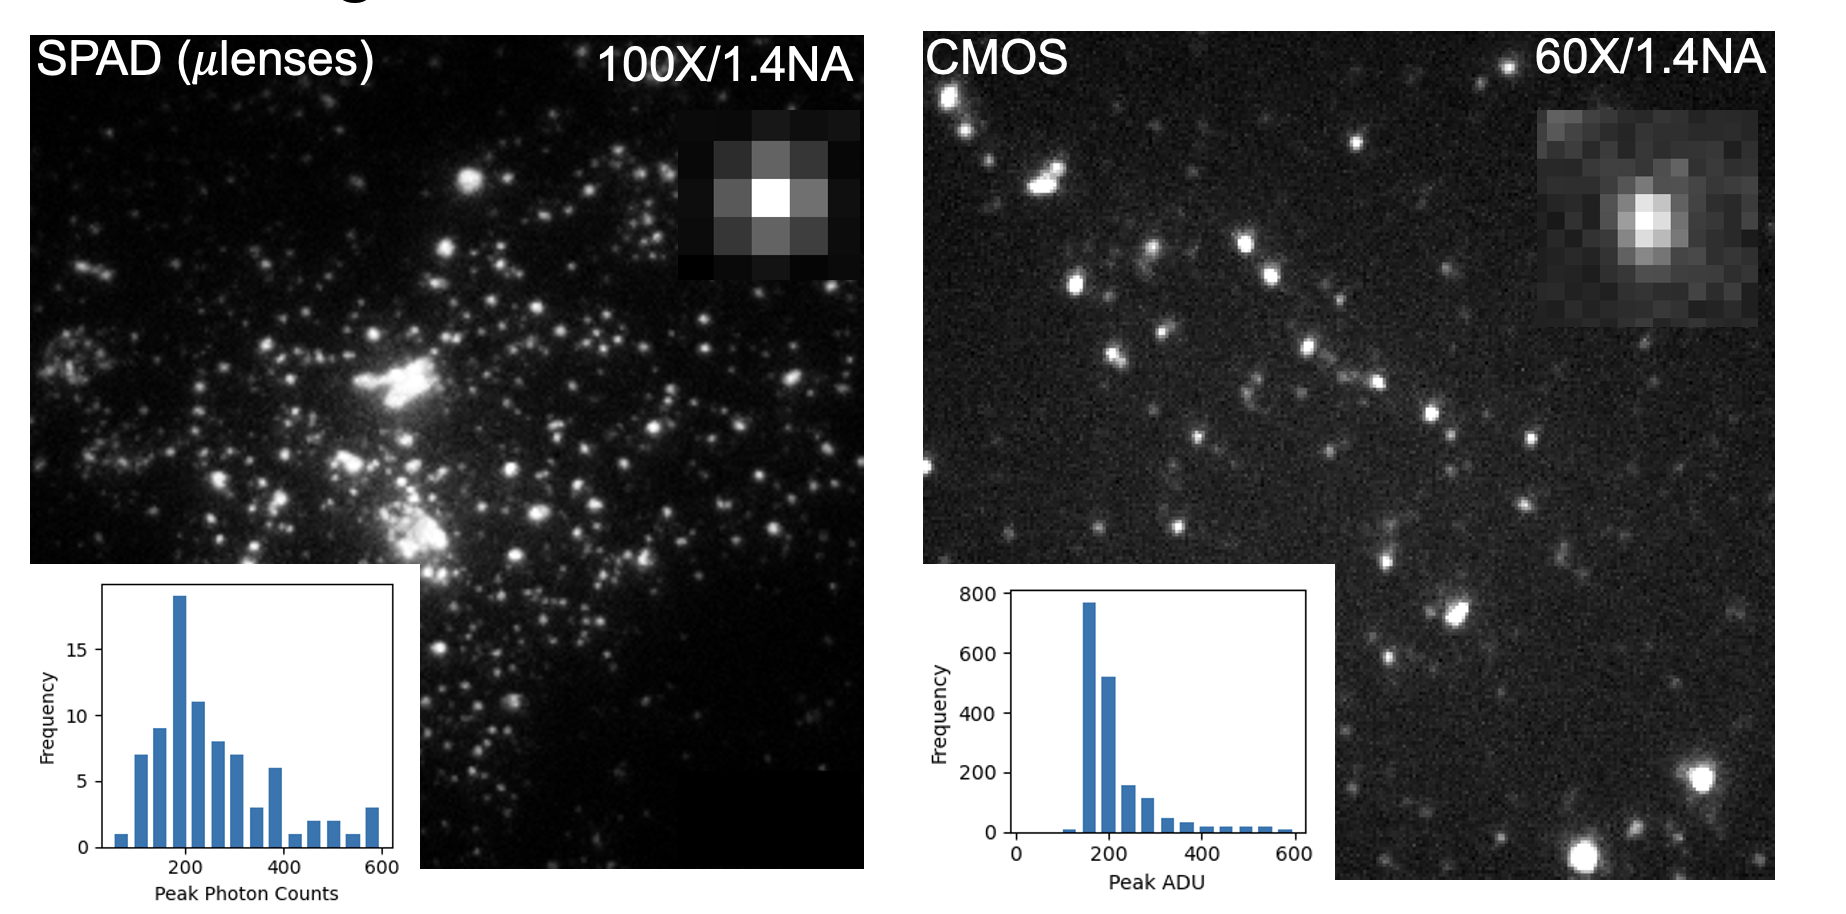
\includegraphics[width=12cm]{SPADvCMOS.png}
\end{figure}
\begin{itemize}
\item SPAD frame is sum of $10^{4}$ 1us exposures
\item This inspires counting molecules in widefield images for enhanced SMLM
\end{itemize}
\end{frame}

\begin{frame}{Counting molecules and enhancing resolution with a SPAD camera}

\begin{textblock*}{11cm}(2.0cm,1.5cm)
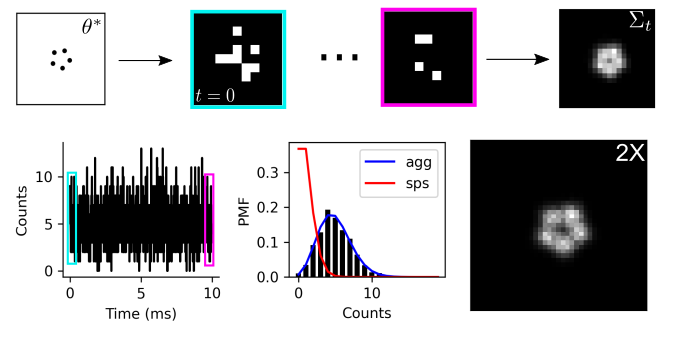
\includegraphics[width=11cm]{DoubleFigure.png}
\end{textblock*}

\begin{textblock*}{11cm}(1cm,7.5cm)
\begin{itemize}
\item Molecular counting for constrained multi-emitter localization
\item Pixel doubling using correlation functions
\end{itemize}

\end{textblock*}


\end{frame}

\begin{frame}{DeepSTORM: Dense SMLM with deep learning}

\begin{textblock*}{12cm}(1cm,1.25cm)
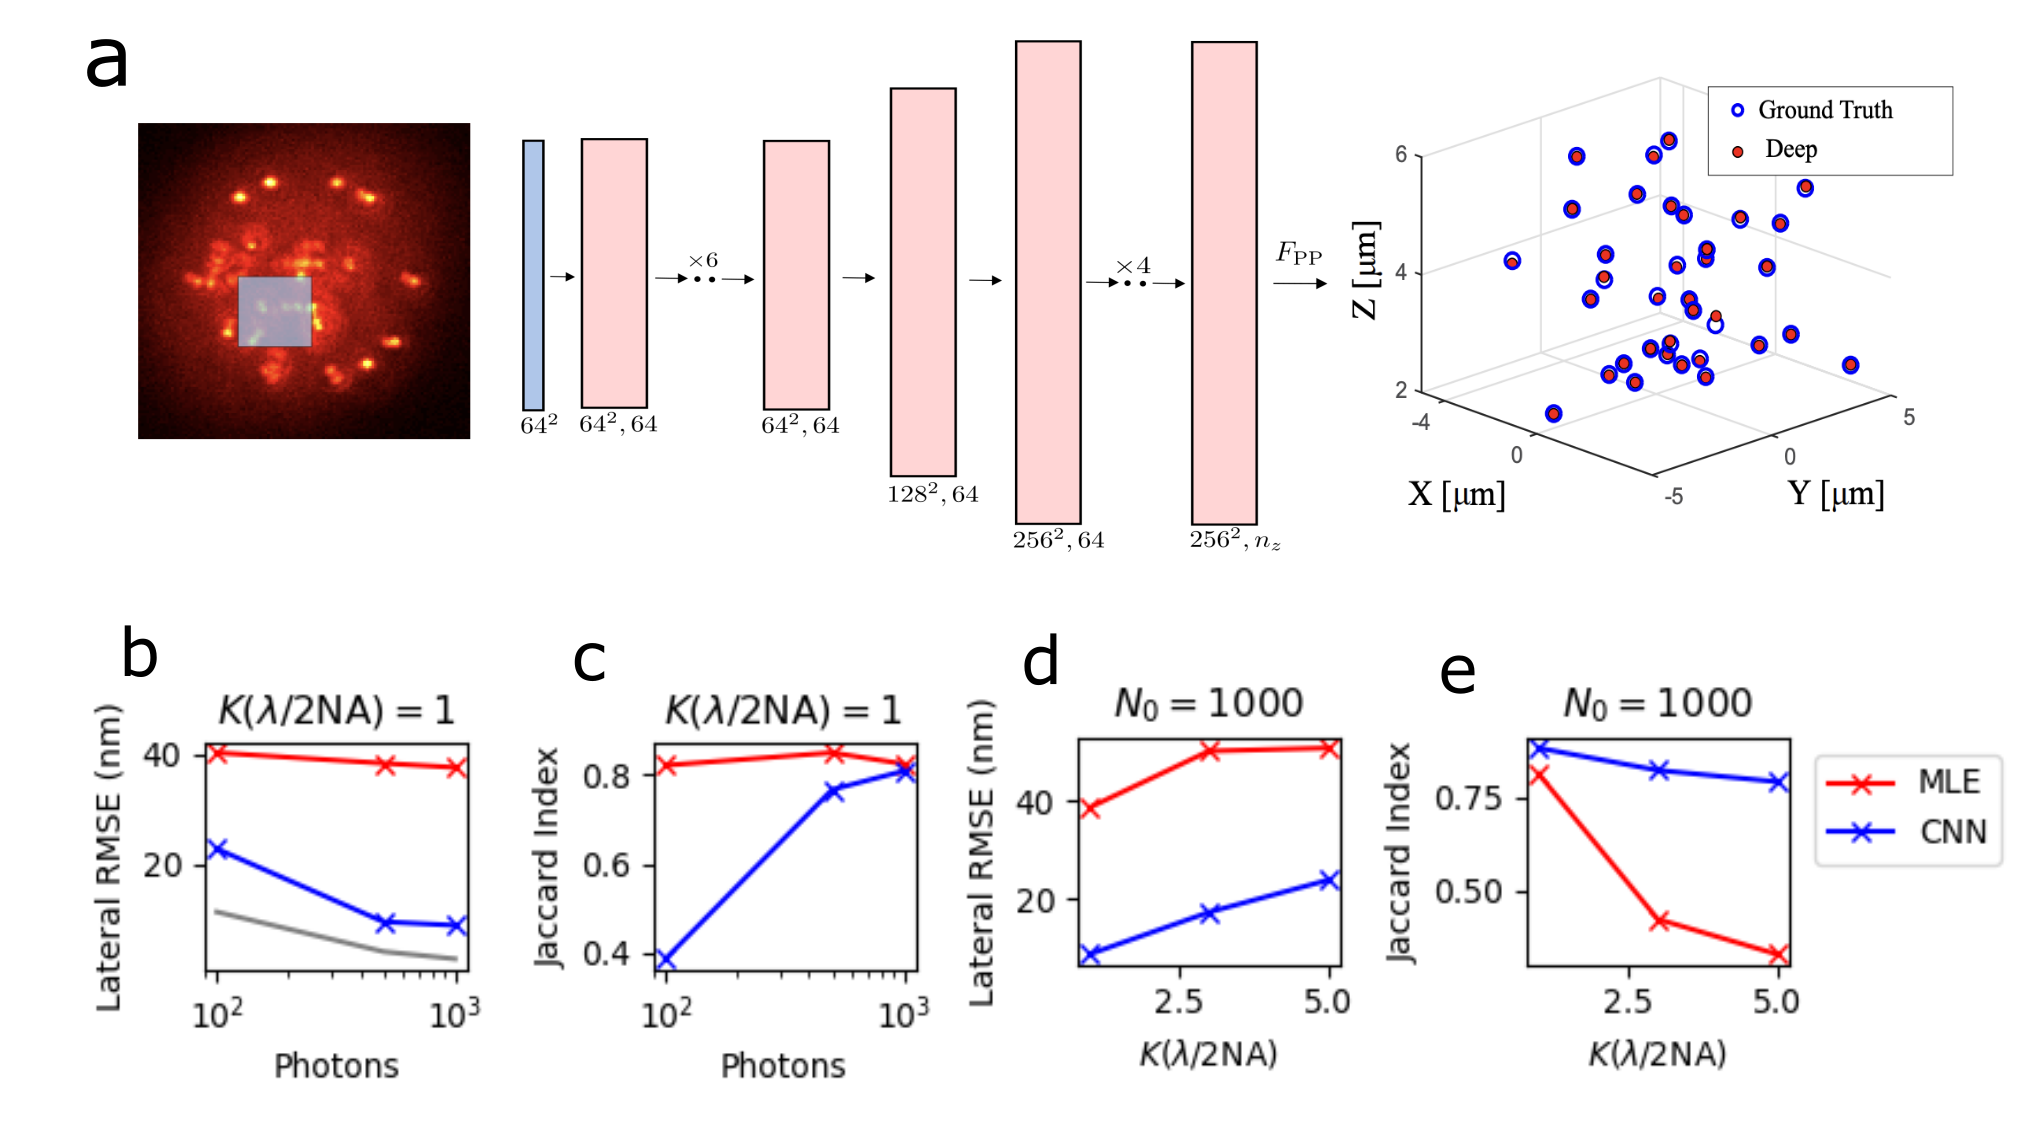
\includegraphics[width=12cm]{PSF2D.png}
\end{textblock*}
\begin{textblock*}{12cm}(1.25cm,8.2cm)
\begin{itemize}
\item MLE in high dimensional spaces can quickly become intractable
\item We can model $P_{\Psi}(\theta_{0})$ with a convolutional neural network $\Psi$
\end{itemize}
\end{textblock*}

\end{frame}

\begin{frame}{Counting molecules and enhancing resolution with a SPAD camera}

\begin{textblock*}{11cm}(2.0cm,1.5cm)
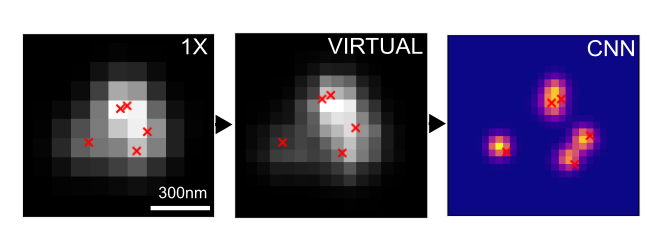
\includegraphics[width=11cm]{Doubled-cNN.png}
Simulated 5 blinking emitters, assigned virtual pixels $\langle X_{i}(t)X_{j}(t) \rangle_{t}$ at or between existing pixels
\end{textblock*}

\begin{textblock*}{11cm}(1cm,7.5cm)
\begin{itemize}
\item On this timescale, relax assumption that $N_{0}$ is constant 
\item For example, photoswitching \textrm{ON} or \textrm{OFF}
\item Fluctuations in $N_{0}$ may be \textbf{uncorrelated} between molecules
\end{itemize}

\end{textblock*}

\end{frame}

\begin{frame}{An integrated method for dense SMLM}
\begin{figure}
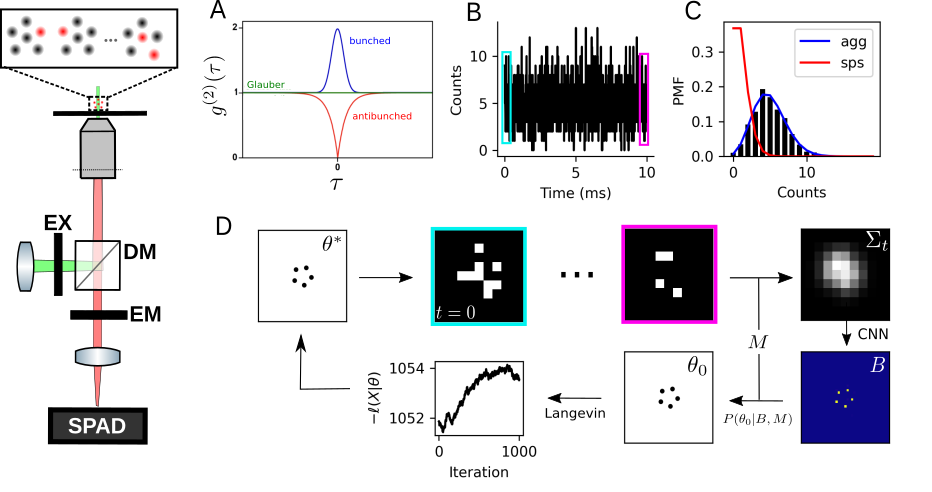
\includegraphics[width=\textwidth]{SPAD.png}
\end{figure}
\begin{itemize}
\item At higher time resolution we can sample from this Poisson PMF 100-1000s of times in a single 10ms exposure
\end{itemize}
\end{frame}


\begin{comment}
\begin{frame}{Chromatin nanodomains in a living Hela cell nucleus}

\begin{textblock*}{13cm}(0.5cm,1.5cm)
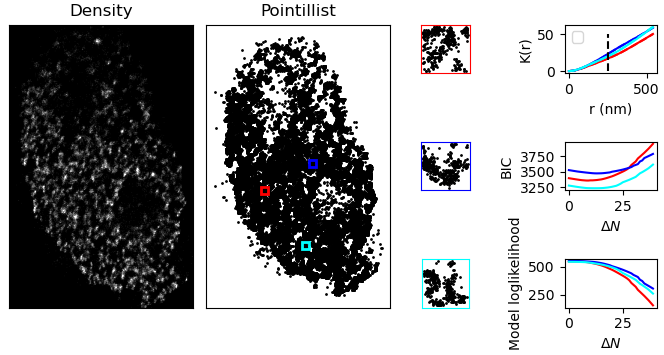
\includegraphics[width=\textwidth]{Cluster.png}
\end{textblock*}

\begin{textblock*}{13cm}(0.5cm,8.0cm)
\begin{itemize}
\item Histone DE using 30x30nm bins
\item Likelihood is computed under a Gaussian Mixture Model (GMM)
\end{itemize}
\end{textblock*}

\end{frame}
\end{comment}


\begin{comment}
\begin{frame}{Next generation SMLM with photon counting cameras}

SOFI techniques conventionally compute autocorrelation functions $G_{ii}^{2}(\bm{r},\tau)$

SOFI images are usually $G^{2}_{ii}(\bm{r},0)$ for each pixel, for long integration times

It is reasonable that $G_{ij}^{2}(\bm{r}_{i},\bm{r}_{j},\tau)$ contains information about molecular positions

\begin{figure}
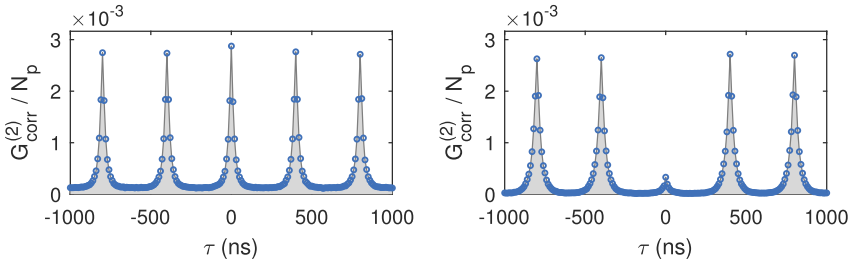
\includegraphics[width=10cm]{G2.png}
\end{figure}

For single photon counts, I don't think $G_{ij}^{2}(\bm{r}_{i},\bm{r}_{j},0)$  contains this information (peaks in $G_{ij}^{2}$ at nonzero lag is evidence for position)
Cross-cumulants may be more appropriate (Girsault 2016), which comes with virtual pixels
May also need pulsed excitation synced with the SPAD camera (can guarantee single photon per molecule per frame)
Higher order correlations might give stronger localization results, but could be intractable to compute (RNNs?)

\end{frame}

\end{comment}

\begin{comment}
\begin{frame}
Now I'm not so sure that the shape of $G_{ij}^{2}$ contains information on position. Translating a molecule along the axes changes the intensity of the individual processes, and I don't believe $G_{ij}^{2}$ is sensitive to the intensity of the processes.
Imagine a molecule emits $N$ photons. As the molecule approaches the neighboring pixel, more photons hit the neighboring pixel, but the delay between consecutive photons hitting pixel 2 and pixel 1 is unchanged. 

However, the intensity information and the anticorrelation of the processes are complementary. The degree of anticorrelated-ness of the various pairs determines how we can "group the pixels". Intensities then could then be used in a full generative model for the data.

A molecule at position $\theta$ will result in anticorrelated neighboring pixels. Perhaps $G_{ij}^{2}(\bm{r}_{i},\bm{r}_{j},0)$ can be use to determine how anti-correlated the pixels are. Then, we use this value to create the "virtual pixels". Then define a likelihood function on the pixels+virtual pixels given the coordinates. 

\end{frame}
\end{comment}

\begin{comment}
\begin{frame}{Dense localization by fluorescence antibunching}

If the emission from a single molecule represents a sub-Poisson process, then the detection process is also sub-Poisson, with a reduced rate. 

Consider point processes $n_{i}(t)$ and $n_{j}(t)$. The second order coherence function reads

\begin{equation*}
g^{2}_{ij}(\tau) = \frac{\langle n_{i}(t+\tau)n_{j}(t)\rangle}{\langle n_{i}(t)\rangle\langle n_{j}(t)\rangle}
\end{equation*}

$n_{i}(t)$ and $n_{j}(t)$ are parameterized by $\theta$. Suppose they are Poisson processes, with rates that can be computed from $\theta$ e.g., $\mu_{i} = f(\theta)$ and $\mu_{j} = g(\theta)$. Then, 

\begin{equation*}
g^{2}_{ij}(0) = \frac{\langle n_{i}(t)n_{j}(t)\rangle}{\mu_{i}\mu_{j}} = 1
\end{equation*}

However, when they are sub-Poisson processes, then $\langle n_{i}(t)n_{j}(t)\rangle \leq \langle n_{i}(t)\rangle\langle n_{j}(t)\rangle$. Why?

The presence of multiple emitters in the local region makes photons appear more ``bunched" w.r.t these two detector elements $i$ and $j$, and therefore $g^{2}_{ij}(0) > 0$. I expect we can use $g^{2}_{ij}(0)$ over 3x3 neighborhoods of pixels where $i$ the center pixel.

\end{frame}
\end{comment}

\begin{comment}
\begin{frame}{Dense localization with fluorescence antibunching}

We require an estimate of emitter locations $\theta^{*}$ to approximate 

\begin{itemize}
\item The number of photons collected in each pixel \\
\item The second order coherence of photon counts in a pixel with its neighbors 
\end{itemize}

Defining a likelihood on the entire time series is intractable. In intensity-based imaging, we would just analyze the sum of photon counts over time. However, the number of emitters is unknown \emph{a priori}, which is part of the problem we are trying to solve. Instead we approximate the maximum likelihood estimate by a stochastic \emph{online parameter estimation} procedure. I imagine emitters are added, if there is not reasonable probability that a photon was emitted by an existing one.

We are able to compute the likelihood of the time summed data and pairwise coherence calculations as the time series and optimization proceed.

\end{frame}
\end{comment}


\begin{comment}
\begin{frame}{Dense localization with fluorescence antibunching}

We need to compute the joint distribution $P(X_{i},X_{j})$. We compute $P(X_{i}=N_{i},X_{j}=N_{j})$ by considering now microstates $\alpha_{i},\alpha_{j}$, which are binary vectors, s.t. $\sum\alpha_{i}=N_{i}$ and $\sum\alpha_{j}=N_{j}$ and have $\alpha_{i}\;\mathrm{AND}\;\alpha_{j}=0$

\begin{align*}
P(X_{i}=N_{i},X_{j}=N_{j}) &\propto \sum_{\alpha,\beta\in \mathcal{A}\otimes \mathcal{B}}\prod_{n}\bm{p}_{i}^{\alpha}\bm{p}_{j}^{\beta}
\end{align*}

But now consider

\begin{equation*}
\langle X_{i}X_{j} \rangle = \sum_{(N_{i},N_{j})} N_{i}N_{j}P(X_{i}=N_{i},X_{j}=N_{j})
\end{equation*}

Antibunching now becomes apparent. If only a single emitter exists (and we have designed $\alpha$'s correctly) then this expectation must be zero for all $(i,j)$.

\end{frame}
\end{comment}


\begin{comment}
\begin{frame}{Chemical fixation changes the appearance of nucleosome clustering}
\begin{textblock*}{12cm}(1.5cm,1.75cm)
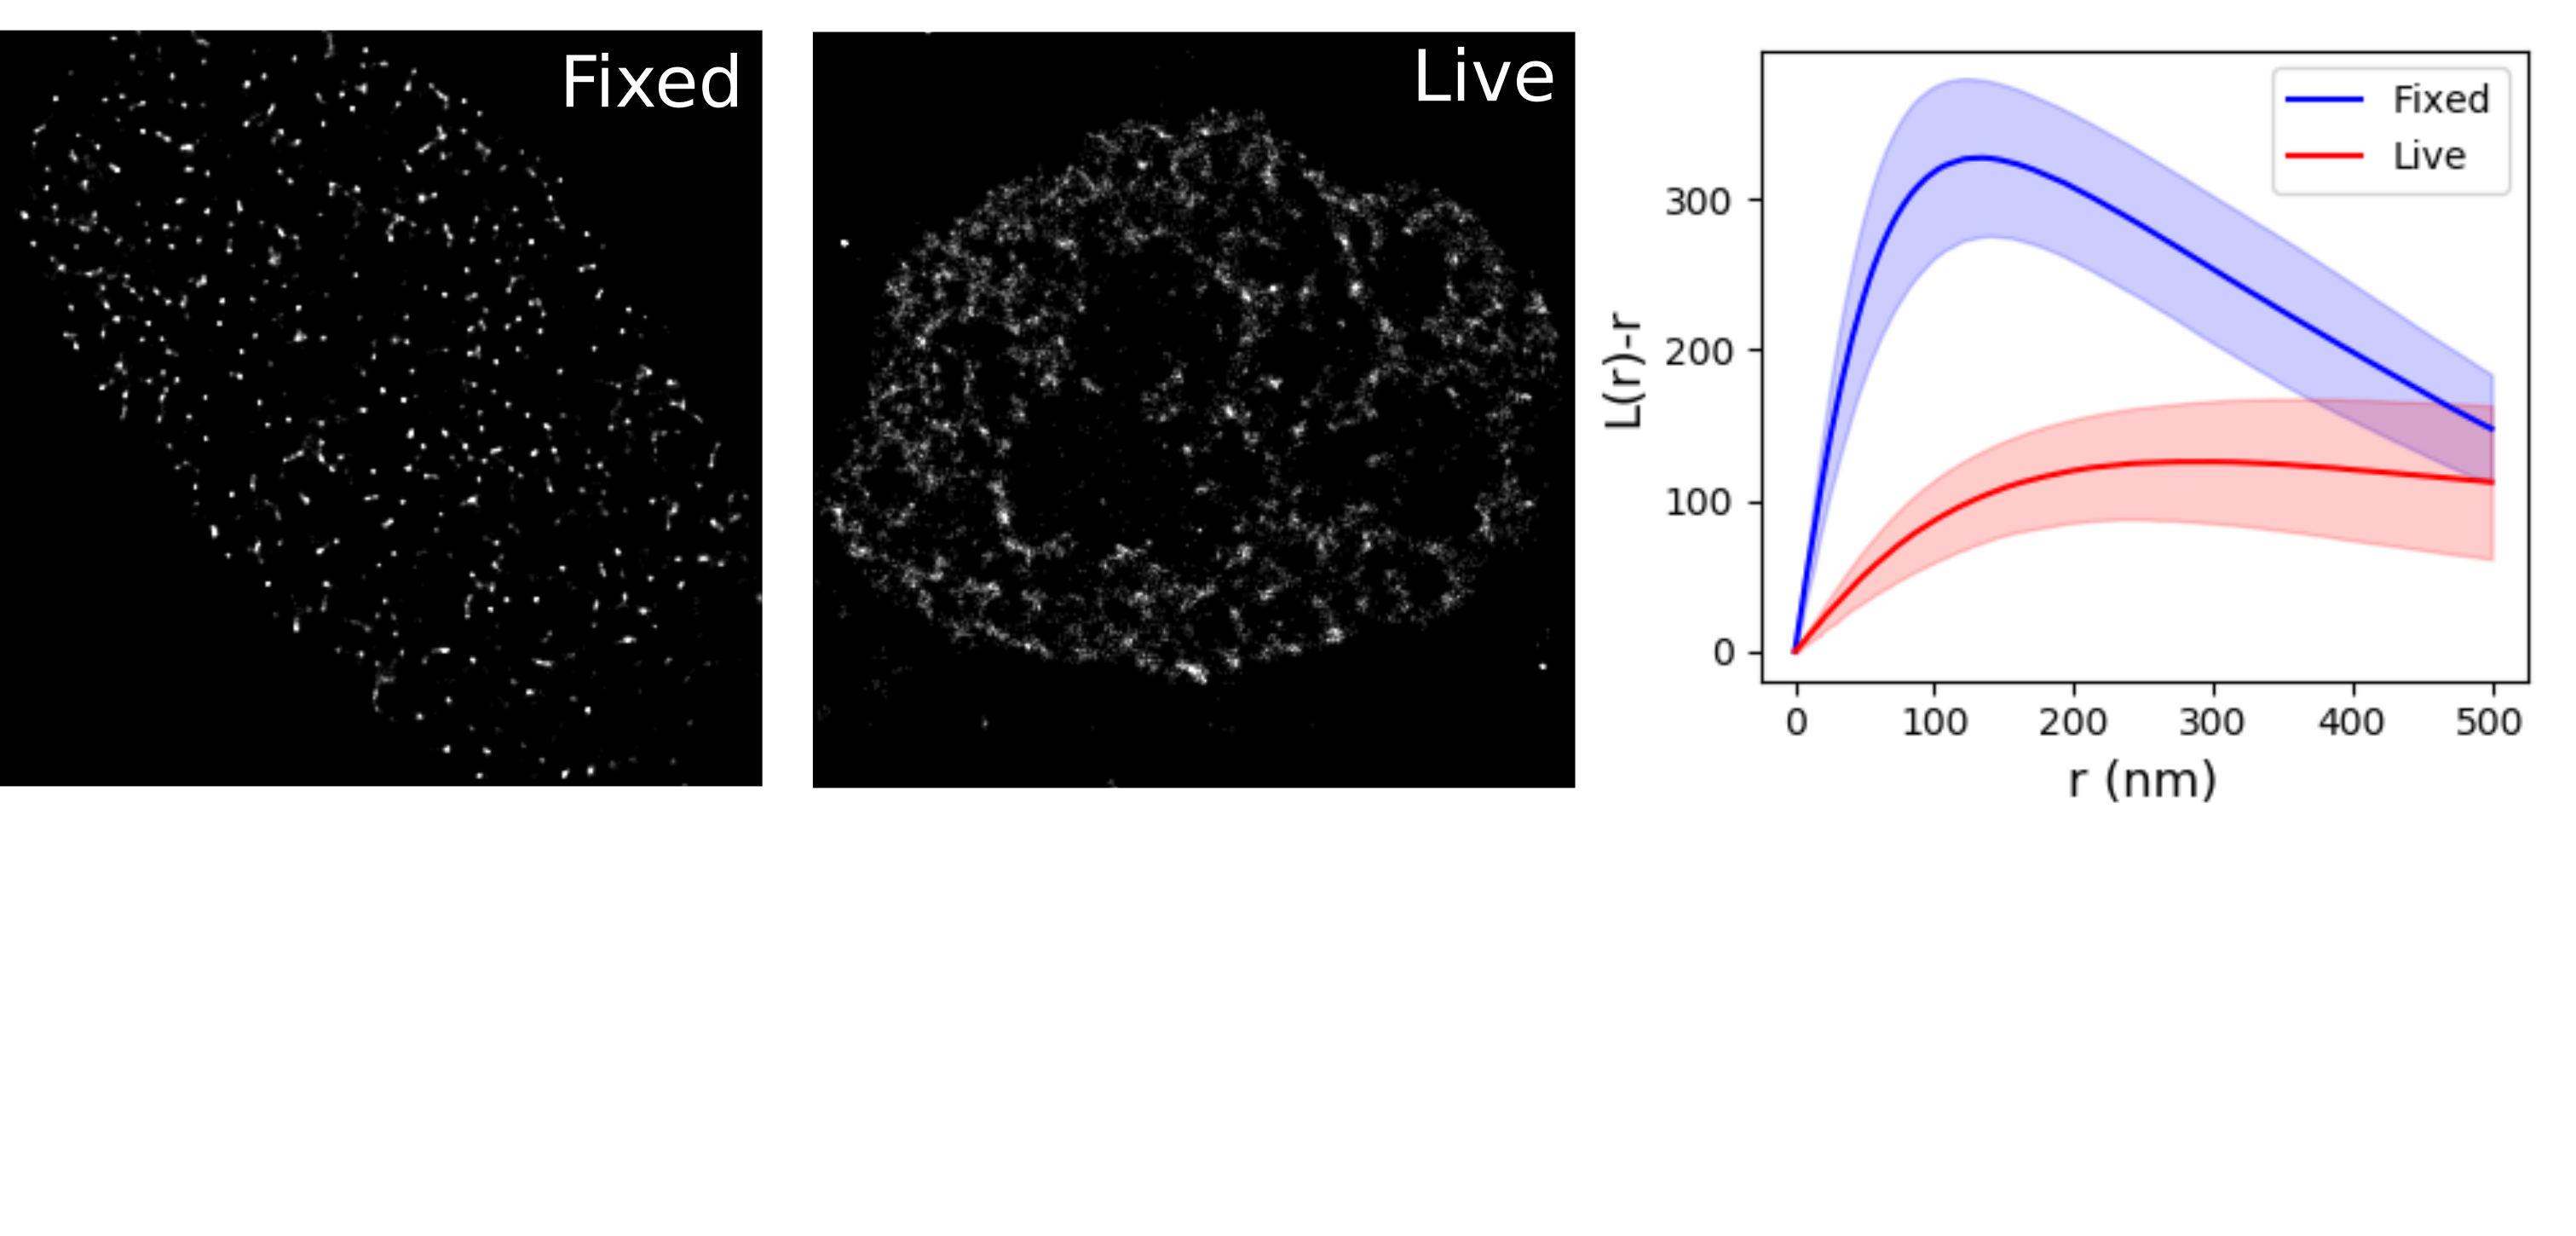
\includegraphics[width=\textwidth]{LiveFix.png}
\end{textblock*}
\end{frame}
\end{comment}

\begin{comment}
\begin{frame}{Astigmatism based three dimensional imaging}
\begin{figure}
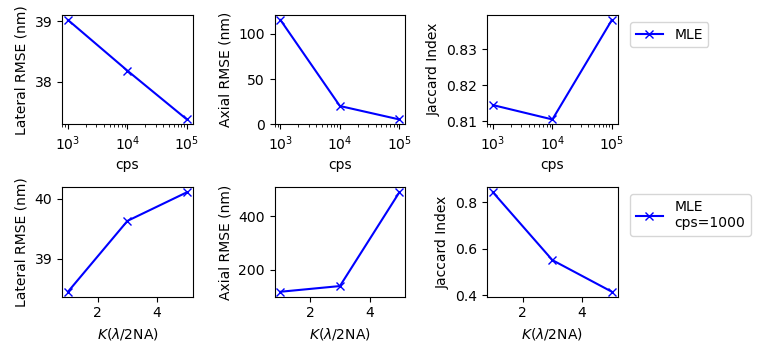
\includegraphics[width=13cm]{PSF3D.png}
\end{figure}
\begin{itemize}
\item $z_{0}\sim U([-0.4,0.4])$ um
\item 3D imaging requires long exposure and sparse emitters for MLE
\item Deep methods may be a suitable choice in future work
\end{itemize}
\end{frame}
\end{comment}

\begin{comment}
\begin{frame}{Astigmatism based three dimensional imaging}
\begin{figure}
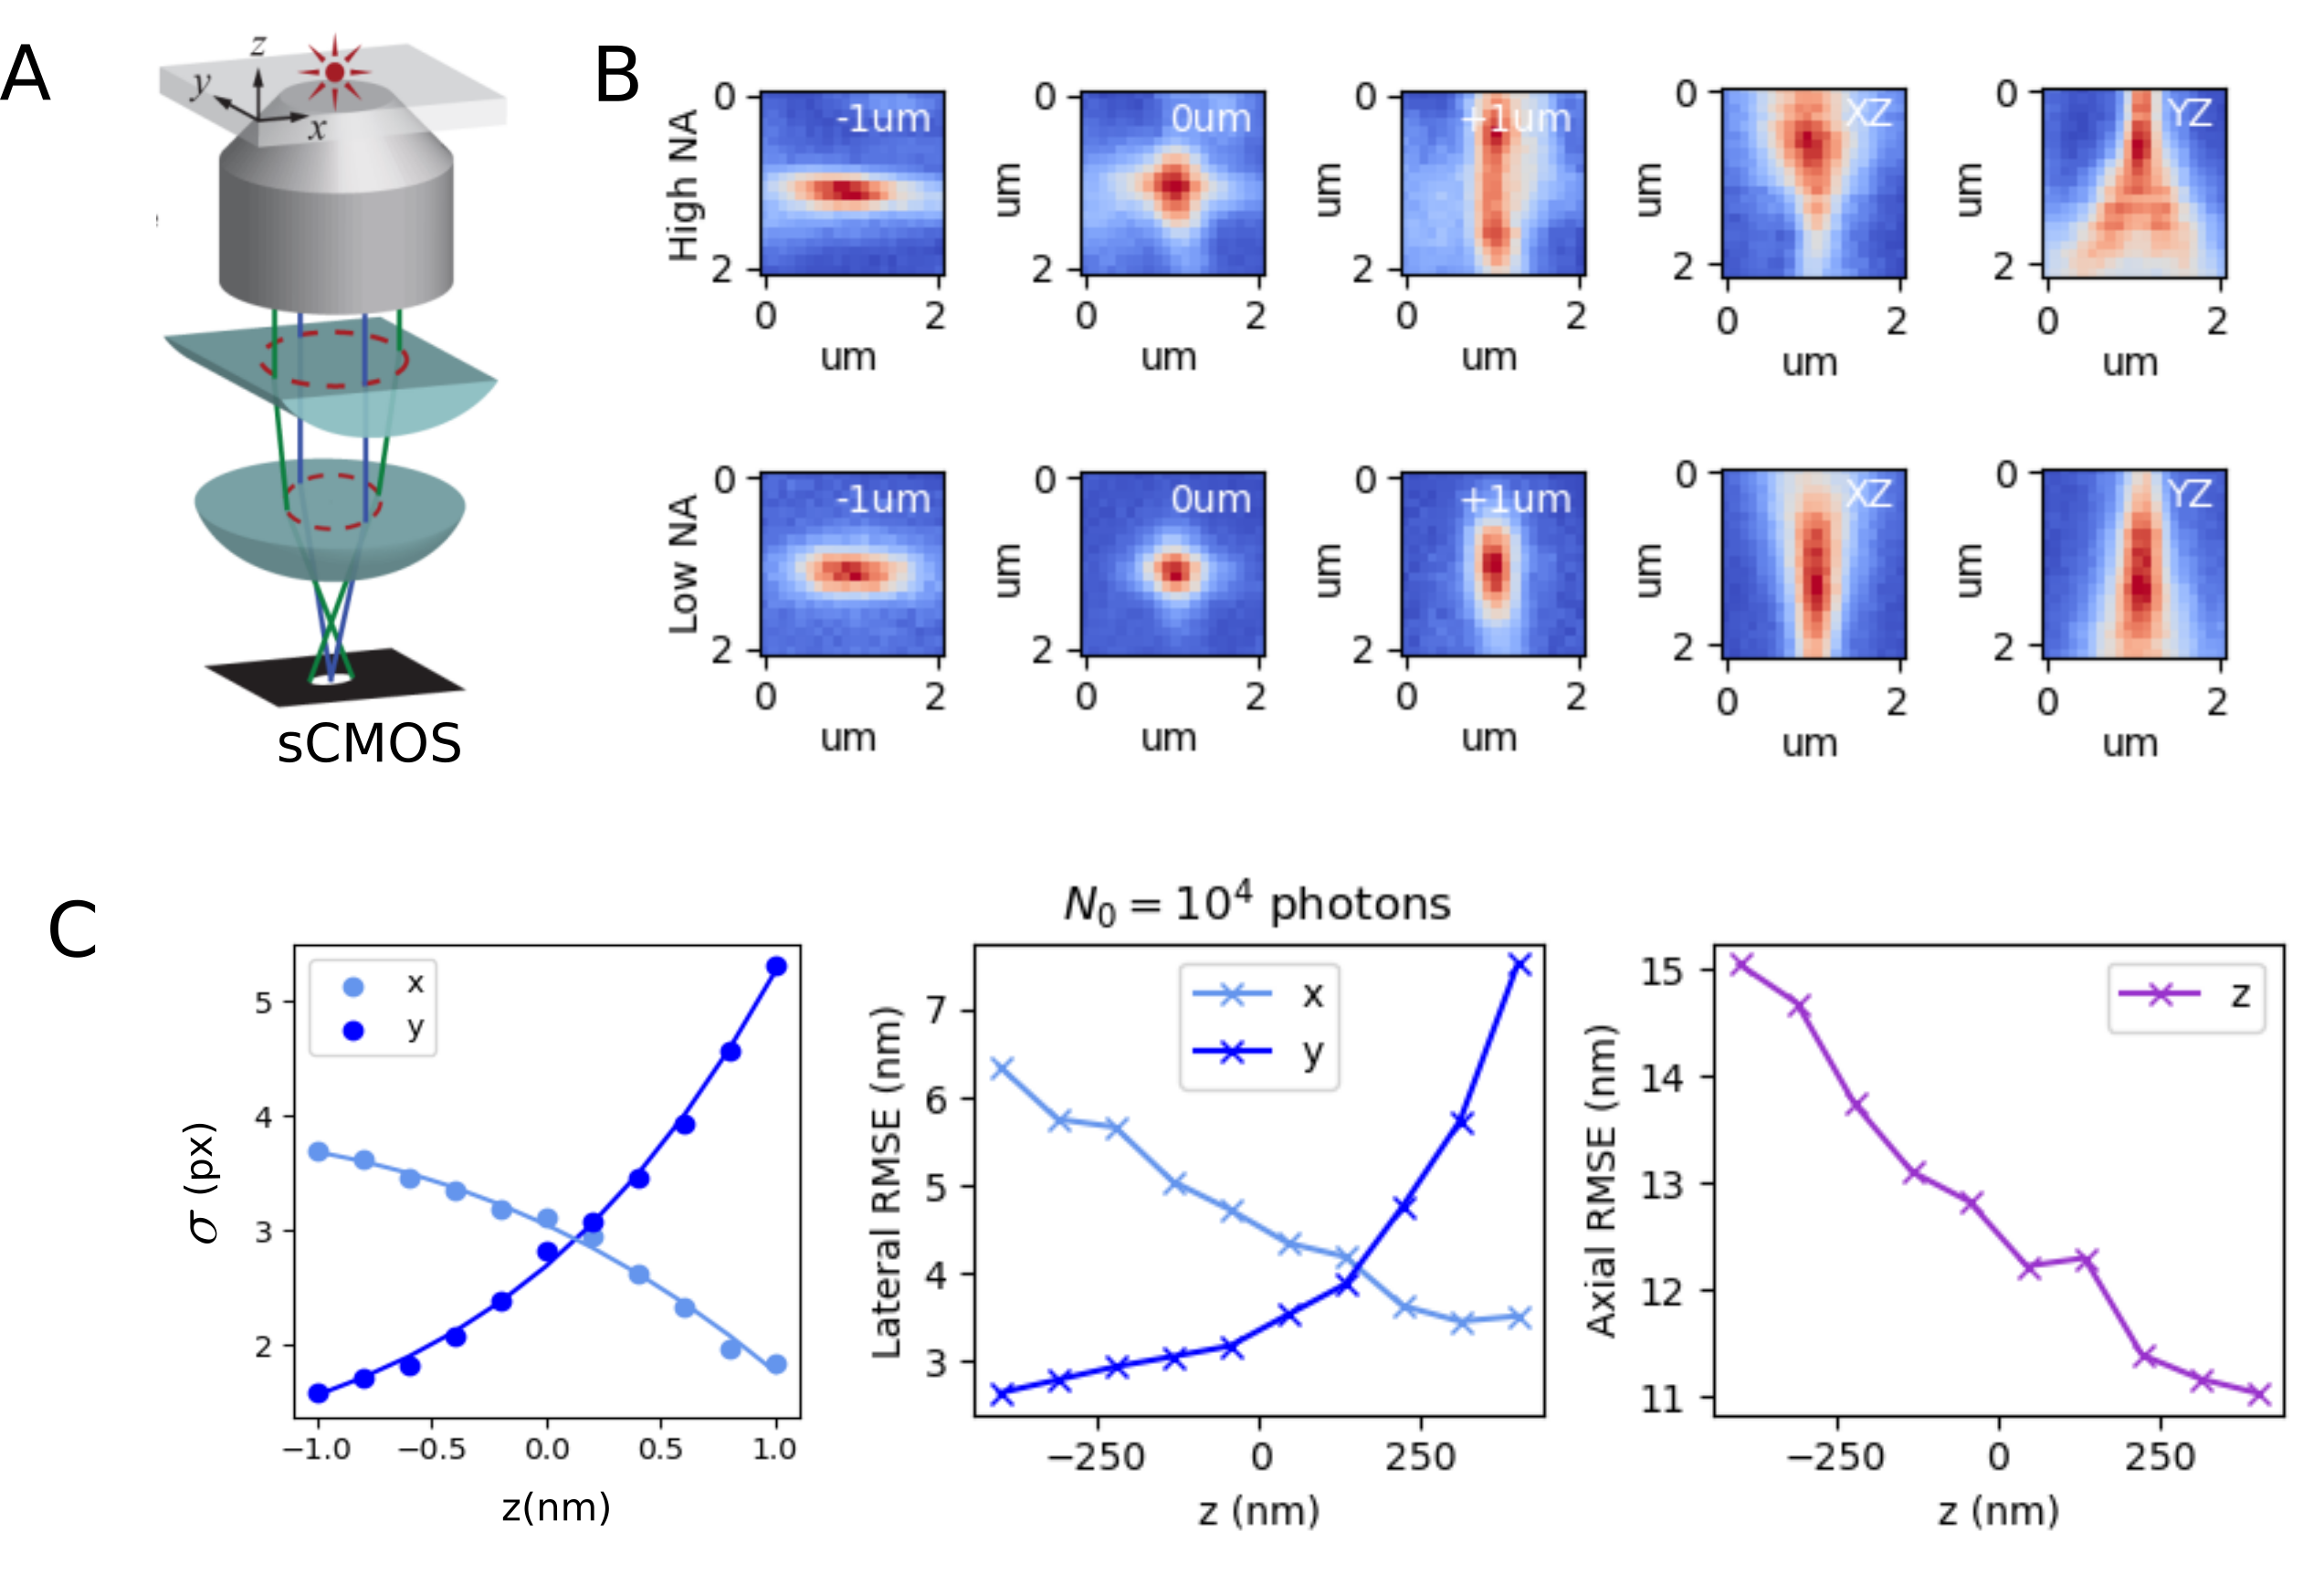
\includegraphics[width=11cm]{Astigmatism.png}
\end{figure}
\begin{itemize}
\item A weak ($f=10$m) cylindrical lens breaks the axial symmetry of the PSF
\end{itemize}
\end{frame}
\end{comment}


\section{Super resolution of chromatin nanodomains}

\begin{comment}
\begin{frame}{Dense labeling of histone H2B in fixed cells at RT}
\begin{textblock*}{11cm}(2.0cm,1.3cm)
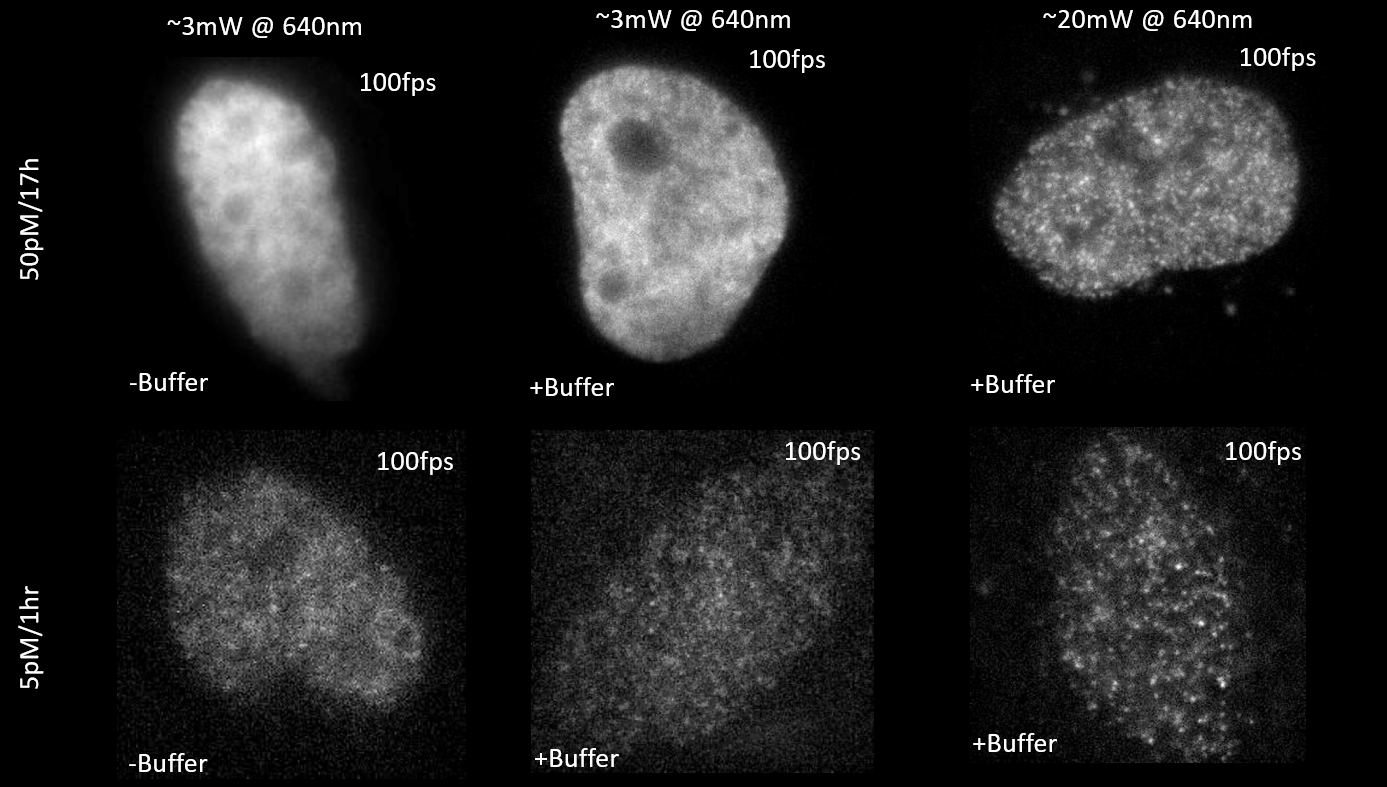
\includegraphics[width=11cm]{Laser.png}
\end{textblock*}
\begin{textblock*}{\textwidth}(0.5cm,8.0cm)
\begin{itemize}
\item Dense labeling of H2B-Halotag w/ fluorescent ligand JF646
\item Reducing buffer is usually a primary thiol like cysteamine (MEA)
\end{itemize}
\end{textblock*}
\end{frame}
\end{comment}

\begin{frame}{Application of dSTORM in living cells}
\begin{textblock*}{12cm}(1.5cm,1.5cm)
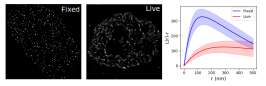
\includegraphics[width=12cm]{LiveFix}
\end{textblock*}
\begin{textblock*}{12cm}(1.0cm,6.5cm)
\begin{itemize}
\item Fixation changes the appearance of nucleosome clustering 
\item Clusters are more dispersed in living cells
\item Dispersion due to nucleosome diffusion and possibly affects of PFA on chromatin architecture
\end{itemize}
\end{textblock*}

\end{frame}



\begin{comment}
\begin{frame}{Chromatin has an intrinsic ability to undergo phase separation}

\begin{textblock*}{10cm}(2.25cm,1.5cm)
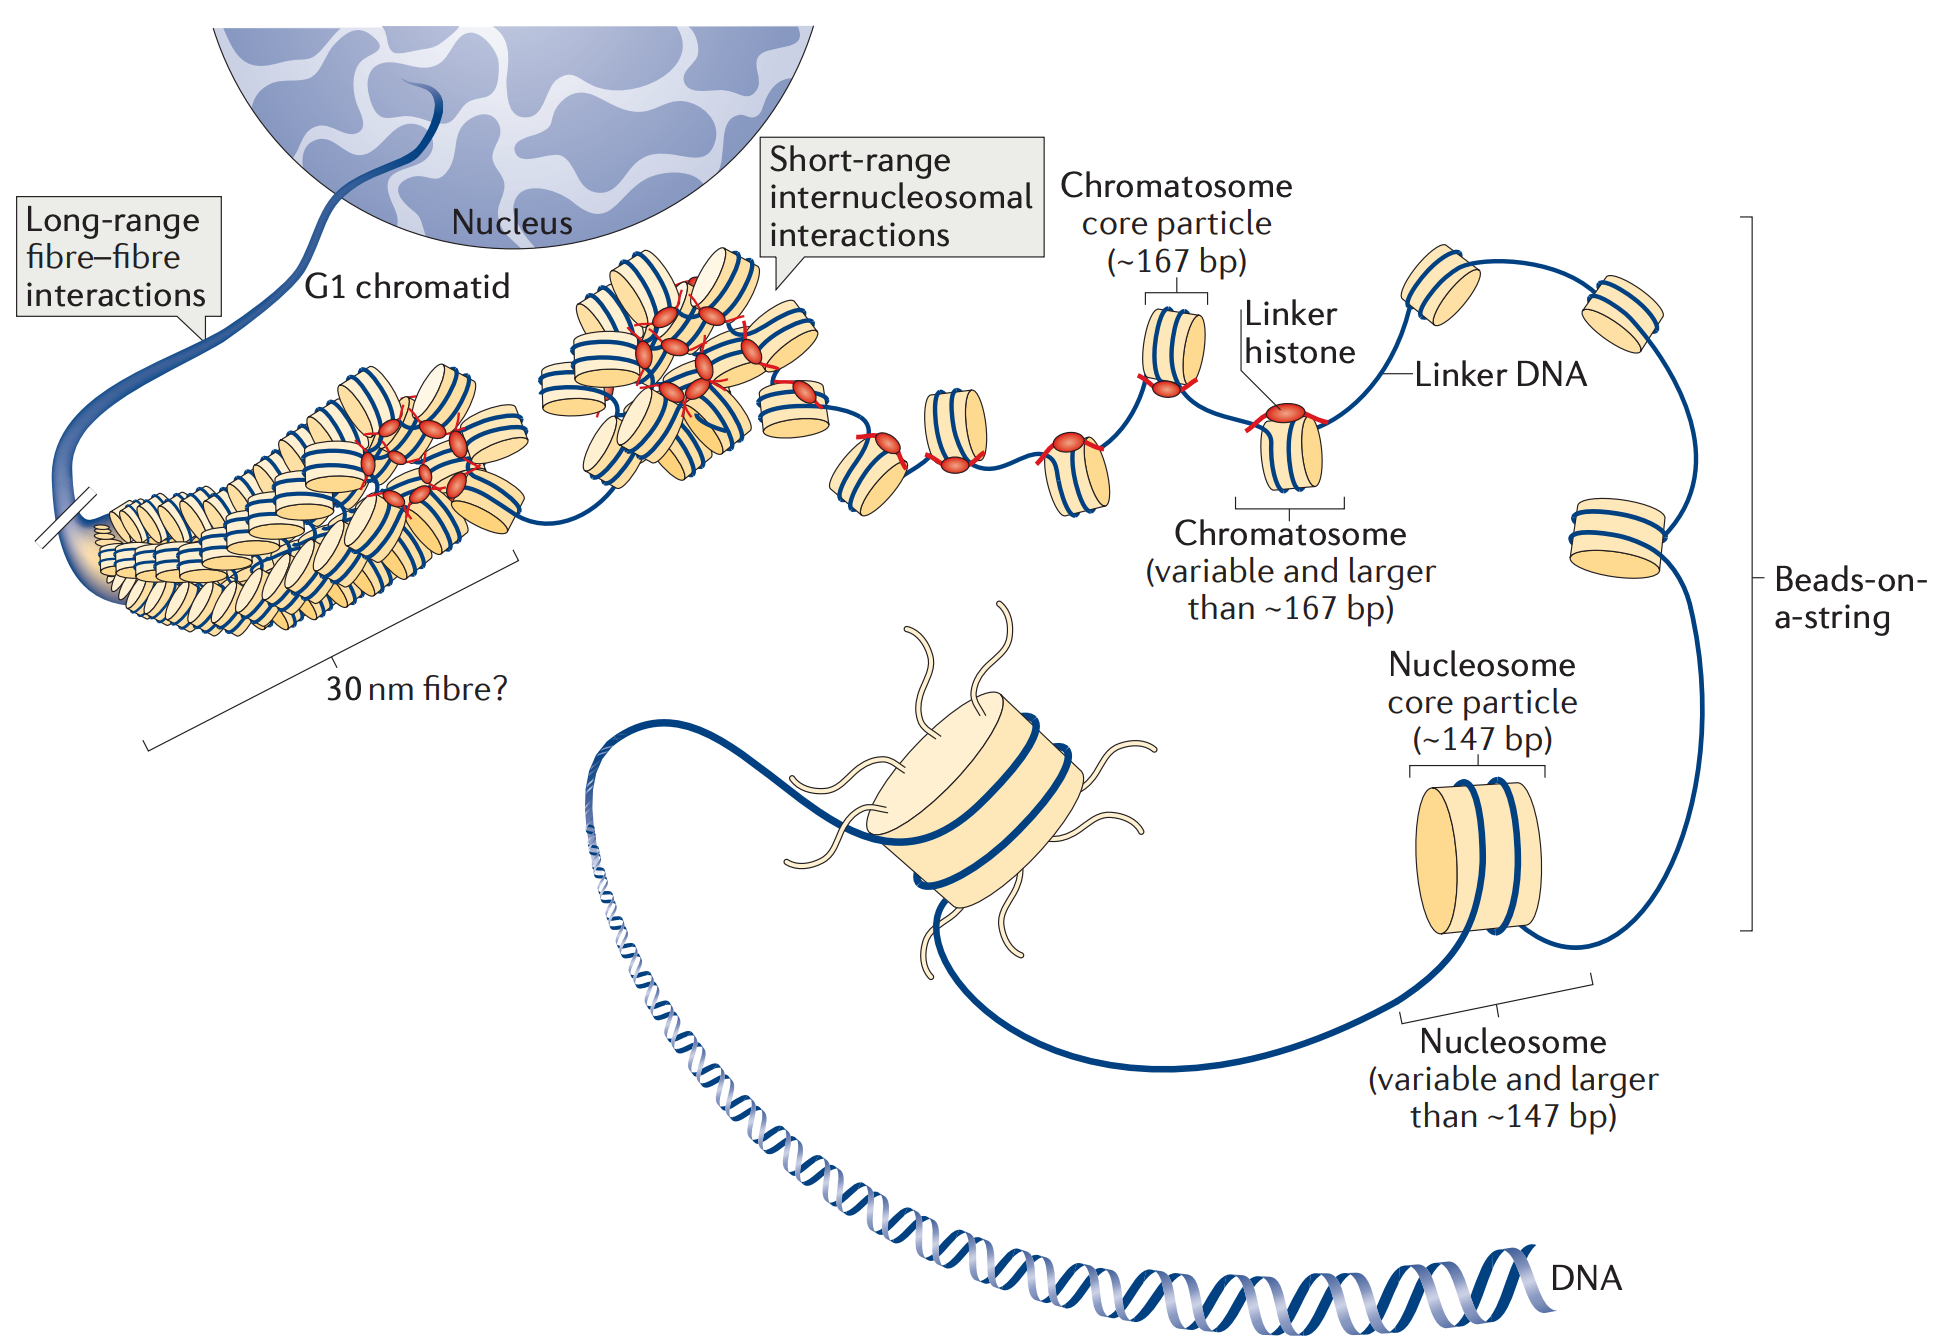
\includegraphics[width=10cm]{Chromatin.png}
\end{textblock*}


\begin{textblock*}{14cm}(0.5cm,7.5cm)
\begin{itemize}
\item Super-enhanced genes are regulated by large molecular assemblies
\item We study nucleosome clustering dynamics using super-resolution microscopy
\end{itemize}
\end{textblock*}

\end{frame}
\end{comment}

\begin{frame}{BRD4 forms phase separated condensates in the nucleus}
\begin{textblock*}{14cm}(0.5cm,1cm)
\begin{figure}
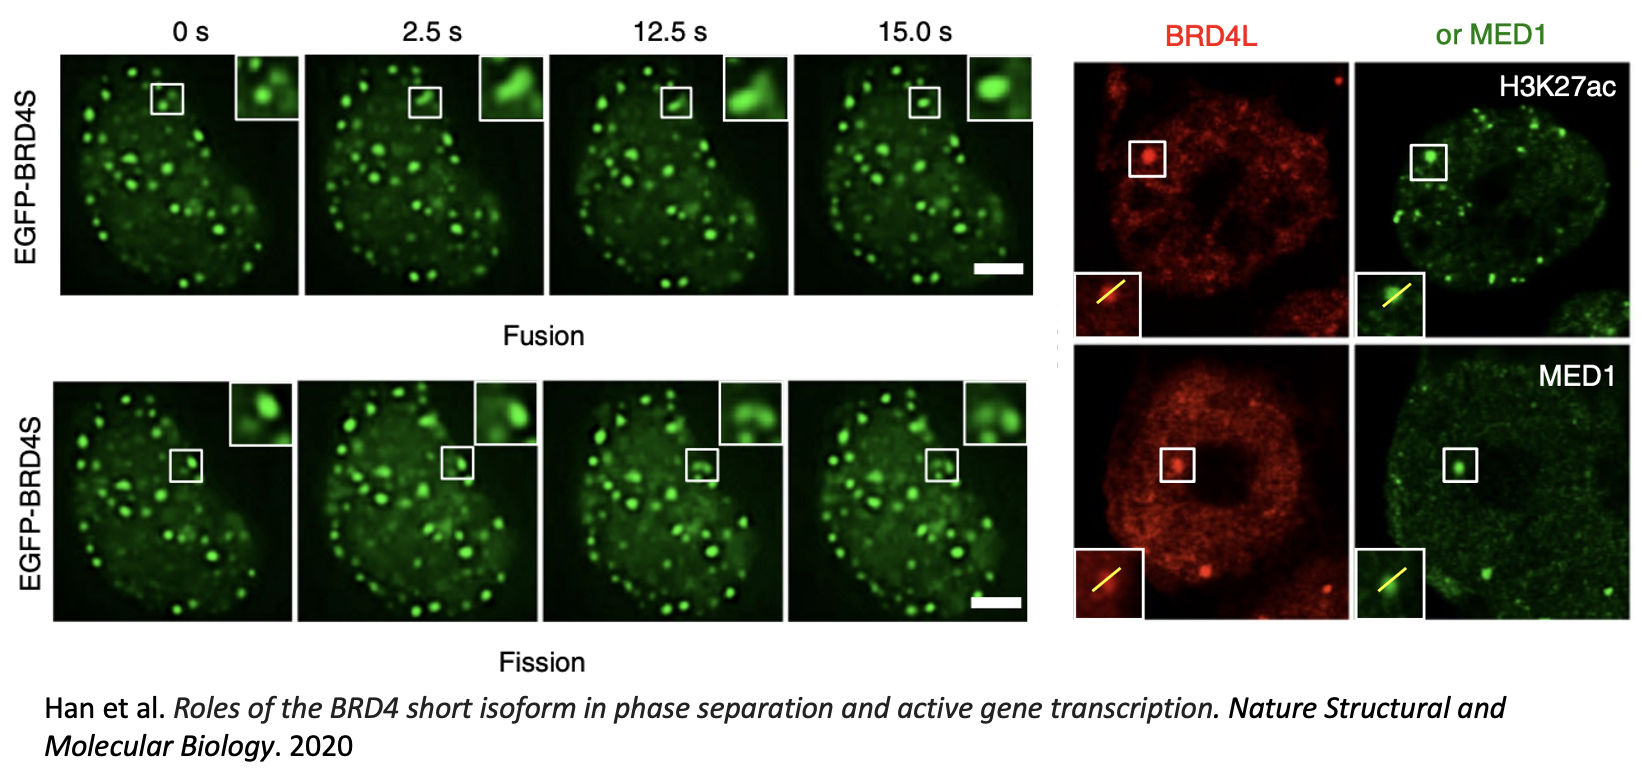
\includegraphics[width=14cm]{Fission.png}
\end{figure}
\end{textblock*}
\end{frame}


\begin{comment}
\begin{frame}{(+)-JQ1 in complex with BRD4 protein}

\begin{textblock*}{6cm}(1.0cm,1.5cm)
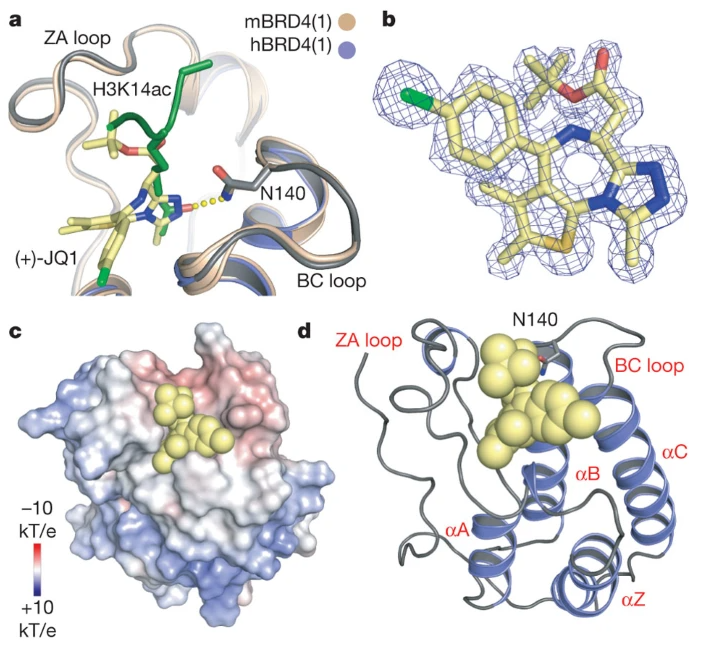
\includegraphics[width=6cm]{JQ1_Complex.png}
\end{textblock*}

\begin{textblock*}{8cm}(7.5cm,1.75cm)
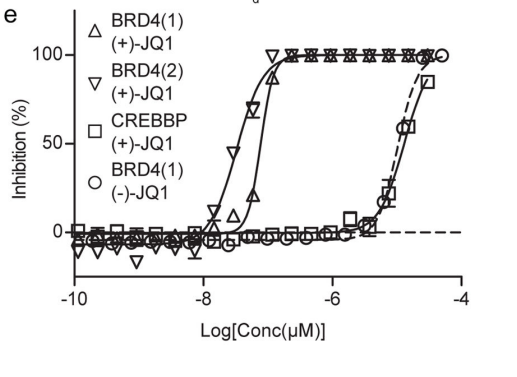
\includegraphics[width=8cm]{BRD4-Inhibition.png}
\end{textblock*}

\begin{textblock*}{\textwidth}(1.0cm,7.5cm)
\textit{Filippakopoulos. Selective inhibition of BET bromodomains. Nature }

\begin{textblock*}{14cm}(0.5cm,8.1cm)
\begin{itemize}
\item BRD4 is an interesting target since specific and non-specific inhibitors exist
\item BET mimics including +JQ1 prevent binding of BRD4 to acetylated histones
\end{itemize}
\end{textblock*}

\end{textblock*}

\end{frame}
\end{comment}

\begin{frame}{Super-resolution of nucleosome-BRD4 interactions in living cells}
\begin{figure}
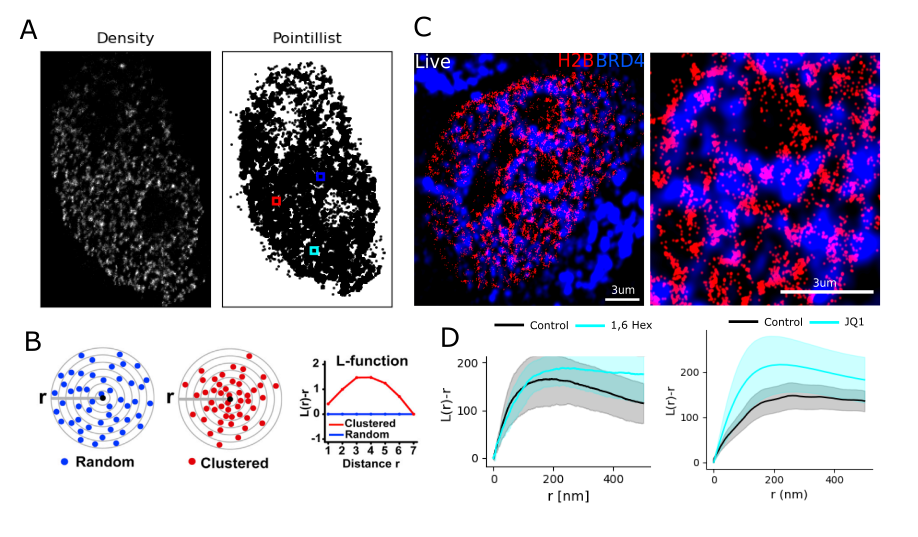
\includegraphics[width=13cm]{BRD4-Results.png}
\end{figure}
\end{frame}


\begin{comment}
\begin{frame}{Inhibition of a super-enhanced gene with JQ1}
\begin{figure}
\includegraphics[width=13cm]{GBP5-1.png}
\end{figure}
Blue - DAPI (binds DNA minor groove)
\begin{itemize}
\item Guanylate binding proteins (GBPs) are a family of GTPases induced by IFN-$\gamma$
\item BRD4 is directly involved in GBP gene expression
\end{itemize}
\end{frame}
\end{comment}


\begin{comment}
\begin{frame}{Inhibition of a super-enhanced gene with JQ1}
\begin{figure}
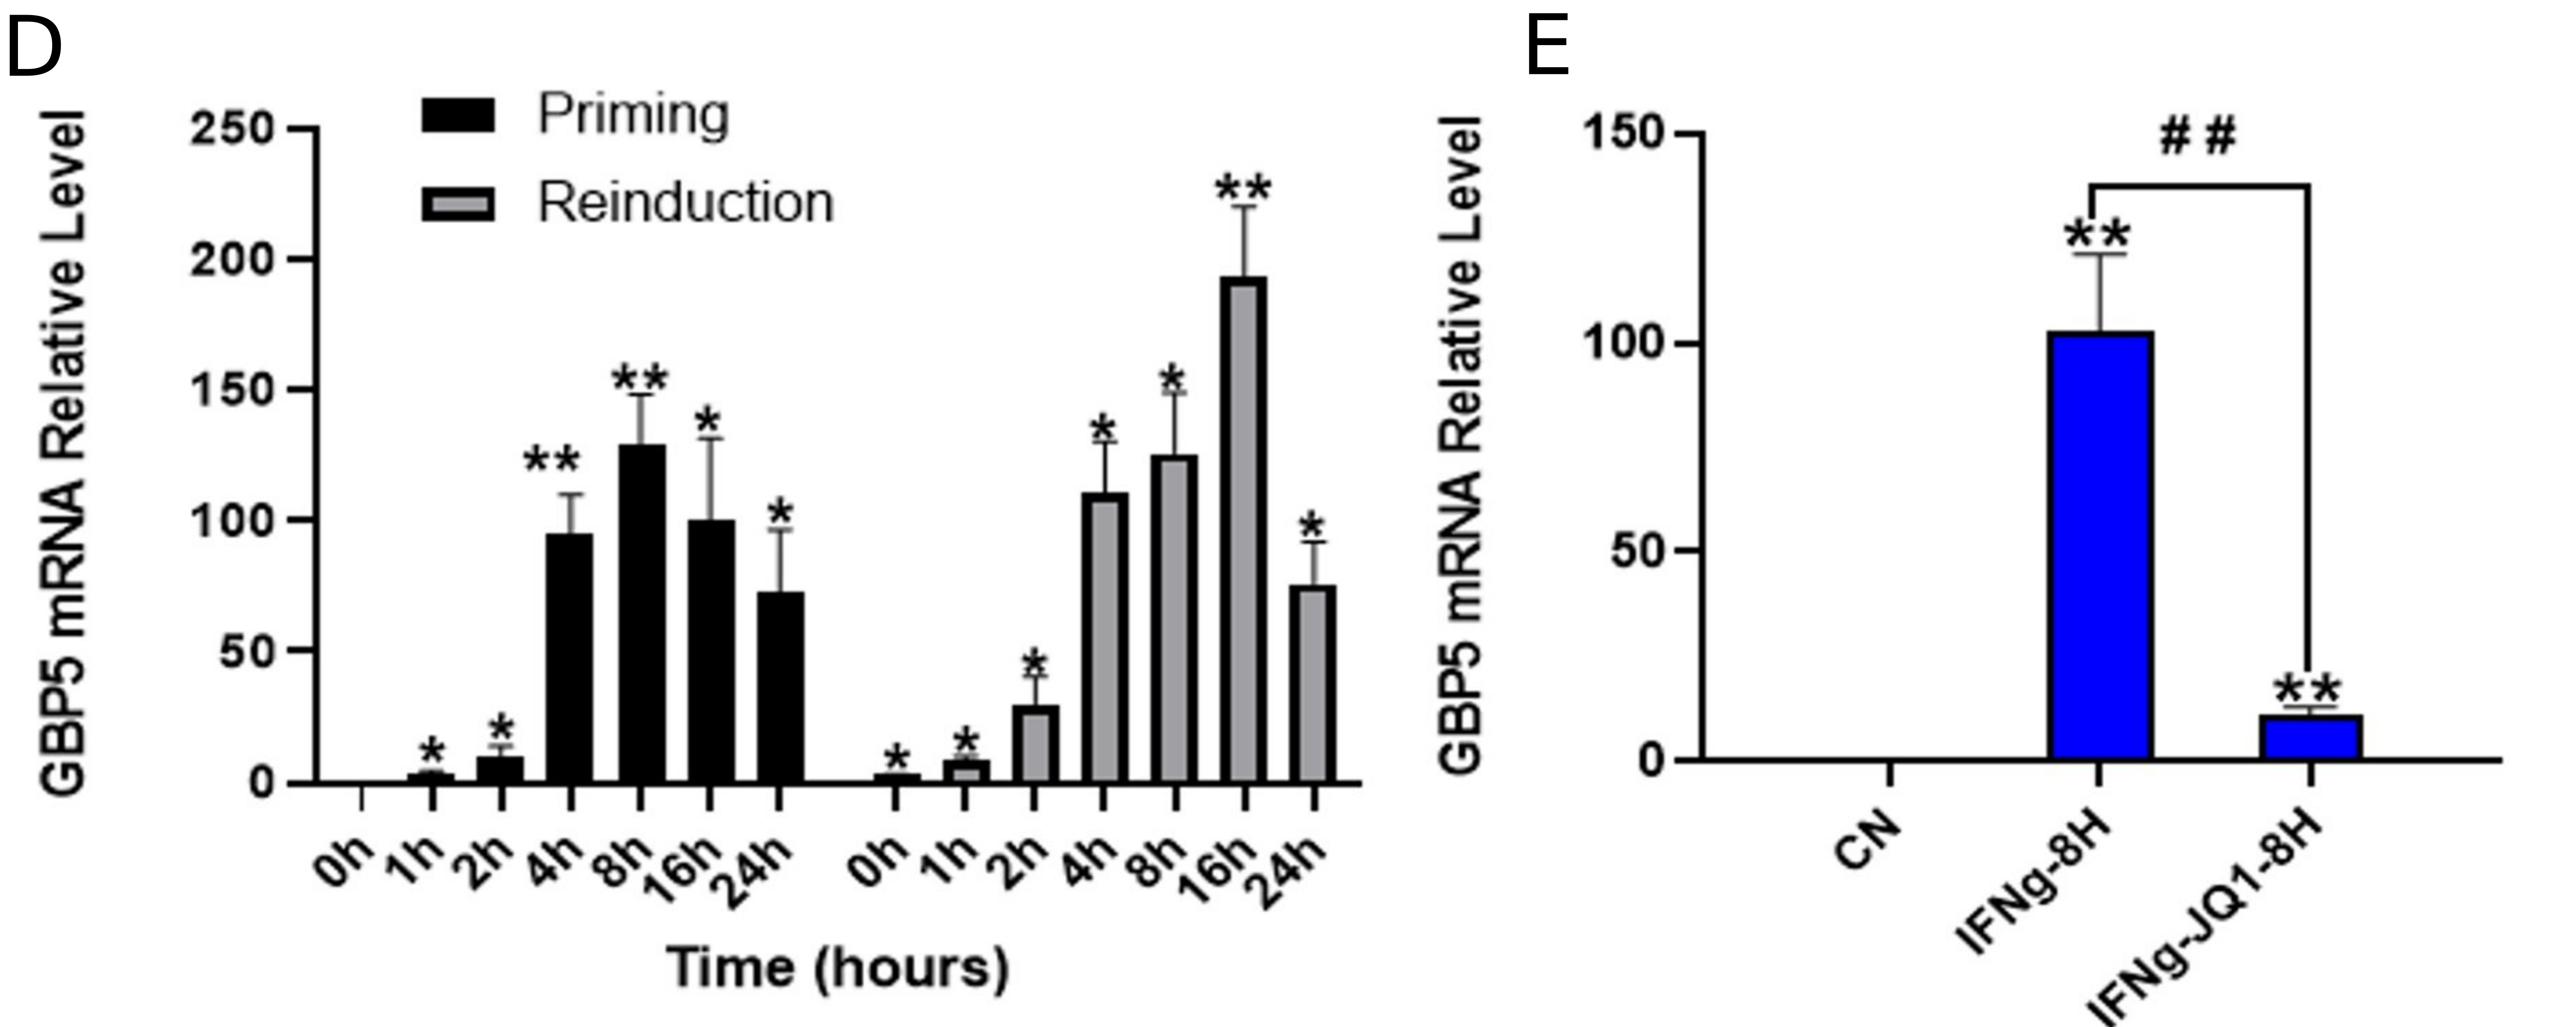
\includegraphics[width=12cm]{GBP5-2.png}
\end{figure}
\begin{itemize}
\item *:$P \leq 0.1$, **:$P \leq 0.01$
\end{itemize}
\end{frame}
\end{comment}

\begin{frame}{Future Aims}
\textbf{Integrate deep models with counting algorithms for enhanced SMLM}
\begin{itemize}
\item Resolution enhancement and counting fluorescent emitters
\end{itemize}
\textbf{Demonstrate that BRD4 phase separates with chromatin and cofactors}
\begin{itemize}
\item BRD4 mutation to inhibit (i) phase separation (ii) chromatin reading function
\item Measure nucleosome diffusion after JQ1 exposure
\end{itemize}
\end{frame}


\begin{frame}{Recent Publications}

\begin{itemize}
\item Seitz et al. \textit{Super-resolution microscopy in-vivo reveals the bromodomain-dependent role of BRD4 in the maintenance of chromatin structure}. \textit{Unpublished}

\item Seitz et al. \textit{Photon counting for enhanced single molecule localization microscopy}. \textit{Unpublished}

\item Maelle Locatelli\textsuperscript{\textdagger}, Josh Lawrimore\textsuperscript{\textdagger}, Hua Lin\textsuperscript{\textdagger}, Sarvath Sanaullah, \textbf{Clayton Seitz}, ..., Pierre-Alexandre Vidi. \textit{DNA damage reduces heterogeneity and coherence of chromatin motions}. PNAS. July 2022\\
\vspace{0.1in}
\item Mengdi Zhang, \textbf{Clayton Seitz}, Garrick Chang, Fadil Iqbal, Hua Lin, and Jing Liu \textit{A guide for single-particle chromatin tracking in live cell nuclei}. Cell Biology International. January 2022.\\
\vspace{0.1in}
\item Wenting Wu, Farooq Syed, Edward Simpson, Chih-Chun Lee, Jing Liu, Garrick Chang, Chuanpeng Dong, \textbf{Clayton Seitz}, ..., Carmella Evans-Molina; \textit{Impact of Proinflammatory Cytokines on Alternative Splicing Patterns in Human Islets}. Diabetes. January 2022
\end{itemize}
\end{frame}

\begin{frame}{Acknowledgements}
\begin{textblock*}{14cm}(0.5cm,1.5cm)
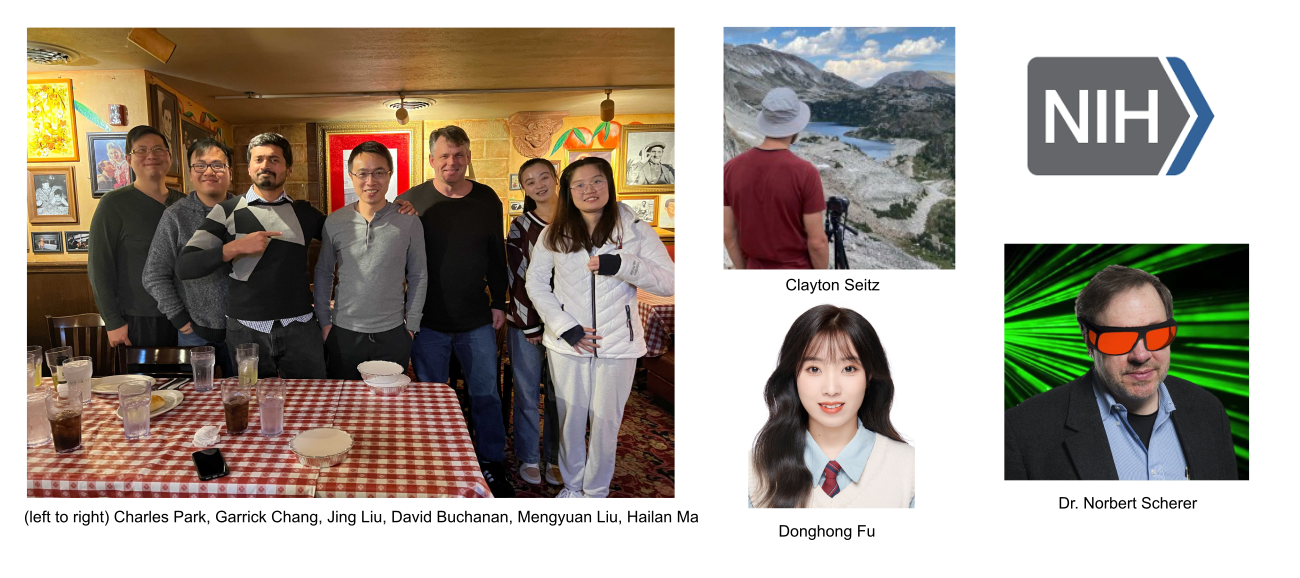
\includegraphics[width=14cm]{Lab.png}
\end{textblock*}

\begin{textblock*}{14cm}(0.5cm,8.5cm)
Thank you!
\end{textblock*}

\end{frame}
\begin{frame}{Selected References}
\noindent [1] Schermelleh, L. et al. \textit{Super-resolution microscopy demystified}. Nature Cell Biology vol. 21 72–84 (2019). 
\newline
\noindent [2] Nehme, E. et al. \textit{DeepSTORM3D: dense 3D localization microscopy and PSF design by deep learning}. Nat Methods 17, 734–740 (2020). 
\newline
\noindent [3] Dertinger, T. et al. \textit{Fast, background-free, 3D super-resolution optical fluctuation imaging (SOFI)}. PNAS
\newline
\noindent [4] Nozaki, T. et al. \textit{Dynamic Organization of Chromatin Domains Revealed by Super-Resolution Live-Cell Imaging}. Mol Cell 67, 282-293.e7 (2017). 
\newline
\noindent [5] Han, X. et al.\textit{ Roles of the BRD4 short isoform in phase separation and active gene transcription}. Nat Struct Mol Biol 27, 333–341 (2020). 
\newline
\end{frame}




\end{document}